\documentclass[review]{igs}
%DIF LATEXDIFF DIFFERENCE FILE
%DIF DEL main_v0.tex   Thu Oct 29 10:39:59 2026
%DIF ADD main_v1.tex   Tue Nov  3 07:13:11 2026

\usepackage[T1]{fontenc}
\usepackage[utf8]{inputenc}
\usepackage{microtype}
\usepackage[english]{babel}
\usepackage{amsmath,amssymb,mathtools,bm}
\usepackage{booktabs,longtable}
\usepackage{graphicx}
\usepackage{enumitem}
\usepackage[authoryear,round]{igsnatbib}

\title[Isochrone overturning]{Isochrone overturning in steady glacier flow}
\author[Lipovsky]{Bradley Paul LIPOVSKY}
\affiliation{Department of Earth and Space Sciences, University of Washington, Seattle, USA\\
Correspondence: Bradley Paul Lipovsky, \texttt{bpl7@uw.edu}}
%DIF PREAMBLE EXTENSION ADDED BY LATEXDIFF
%DIF UNDERLINE PREAMBLE %DIF PREAMBLE
\RequirePackage[normalem]{ulem} %DIF PREAMBLE
\RequirePackage{color}\definecolor{RED}{rgb}{1,0,0}\definecolor{BLUE}{rgb}{0,0,1} %DIF PREAMBLE
\providecommand{\DIFadd}[1]{{\protect\color{blue}\uwave{#1}}} %DIF PREAMBLE
\providecommand{\DIFdel}[1]{{\protect\color{red}\sout{#1}}}                      %DIF PREAMBLE
%DIF SAFE PREAMBLE %DIF PREAMBLE
\providecommand{\DIFaddbegin}{} %DIF PREAMBLE
\providecommand{\DIFaddend}{} %DIF PREAMBLE
\providecommand{\DIFdelbegin}{} %DIF PREAMBLE
\providecommand{\DIFdelend}{} %DIF PREAMBLE
\providecommand{\DIFmodbegin}{} %DIF PREAMBLE
\providecommand{\DIFmodend}{} %DIF PREAMBLE
%DIF FLOATSAFE PREAMBLE %DIF PREAMBLE
\providecommand{\DIFaddFL}[1]{\DIFadd{#1}} %DIF PREAMBLE
\providecommand{\DIFdelFL}[1]{\DIFdel{#1}} %DIF PREAMBLE
\providecommand{\DIFaddbeginFL}{} %DIF PREAMBLE
\providecommand{\DIFaddendFL}{} %DIF PREAMBLE
\providecommand{\DIFdelbeginFL}{} %DIF PREAMBLE
\providecommand{\DIFdelendFL}{} %DIF PREAMBLE
%DIF COLORLISTINGS PREAMBLE %DIF PREAMBLE
\RequirePackage{listings} %DIF PREAMBLE
\RequirePackage{color} %DIF PREAMBLE
\lstdefinelanguage{DIFcode}{ %DIF PREAMBLE
%DIF DIFCODE_UNDERLINE %DIF PREAMBLE
  moredelim=[il][\color{red}\sout]{\%DIF\ <\ }, %DIF PREAMBLE
  moredelim=[il][\color{blue}\uwave]{\%DIF\ >\ } %DIF PREAMBLE
} %DIF PREAMBLE
\lstdefinestyle{DIFverbatimstyle}{ %DIF PREAMBLE
	language=DIFcode, %DIF PREAMBLE
	basicstyle=\ttfamily, %DIF PREAMBLE
	columns=fullflexible, %DIF PREAMBLE
	keepspaces=true %DIF PREAMBLE
} %DIF PREAMBLE
\lstnewenvironment{DIFverbatim}{\lstset{style=DIFverbatimstyle}}{} %DIF PREAMBLE
\lstnewenvironment{DIFverbatim*}{\lstset{style=DIFverbatimstyle,showspaces=true}}{} %DIF PREAMBLE
%DIF END PREAMBLE EXTENSION ADDED BY LATEXDIFF

\begin{document}
\DIFdelbegin %DIFDELCMD < \abstract{Ancient ice recovered at Allan Hills extends into the Miocene, but steep layers, age reversals and folds complicate its interpretation. Whether steady glacier flow can overturn initially ordered layers remains uncertain. Here, we track the horizontal order of particles deposited sequentially at the surface. This order is measured by a signed Jacobian that is equivalent to the inverse vertical-thinning factor while layers remain ordered. We find that overturning depends directly on the cumulative competition between vertical shear, which preserves depositional order, and reverse shear, which erodes it. Reverse shear accumulates faster where horizontal speed is small. A layer becomes vertical only after reverse shear has erased both its initial ordering and the ordering accumulated during earlier flow. Full-Stokes mechanics does not guarantee preservation, although shallow-ice flow does. We derive an overturning threshold, bounds for localized obstacles, a cancellation result for periodic bed roughness and a trajectory-based diagnostic for numerical models. Gravity-driven full-Stokes flow with a linear sliding law generates recumbent folding directly from ordered surface deposition, without inherited disturbance or time dependence. Layer curvature and topographic draping can occur without order reversal; the Jacobian provides a test of steady-flow explanations of disturbed stratigraphy at Allan Hills and other old-ice sites.}
%DIFDELCMD < %%%
\DIFdelend \DIFaddbegin \abstract{Ancient ice recovered at Allan Hills extends into the Miocene, but steep layers, age reversals and folds complicate its interpretation. Whether steady glacier flow can overturn initially ordered layers remains uncertain. Here, we track the horizontal order of particles deposited sequentially at the surface. This order is measured by a signed Jacobian that is equivalent to the inverse vertical-thinning factor while layers remain ordered. We find that overturning depends directly on the cumulative competition between vertical shear, which preserves depositional order, and reverse shear, which erodes it. Reverse shear accumulates faster where horizontal speed is small. A layer becomes vertical only after reverse shear has erased both its initial ordering and the ordering accumulated during earlier flow. The full-Stokes equations supply no general sign-preservation result, although shallow-ice flow does. We derive an overturning threshold, bounds for localized obstacles, a cancellation result for periodic bed roughness and trajectory-based diagnostics for numerical models. A finite convergent point-margin flow reverses an ordered incoming material line under its stated boundary closure, whereas 750 resolved periodic sinusoidal-bed calculations preserve surface-deposition order. Layer curvature and topographic draping can occur without order reversal; the Jacobian provides a test of steady-flow explanations of disturbed stratigraphy at Allan Hills and other old-ice sites.}
\DIFaddend

\maketitle

\noindent\textbf{Keywords:} glacier flow; ice stratigraphy; recumbent folds; blue ice; full-Stokes modelling

\section{Introduction}

Recovering old ice is useful only where its age and stratigraphic context can be established. At Little Dome C, radar and flow modelling have been used to target a continuous record beyond \(1~\mathrm{Ma}\) \citep{Lilien2021,Chung2025BeyondEPICA}. Antarctic blue-ice areas instead expose discontinuous intervals through surface ablation and upward ice motion \citep{Bintanja1999,Spaulding2012}. The S{\o}r Rondane Mountains are another blue-ice setting being surveyed for old ice \citep{Izeboud2026}. At Allan Hills, cores have progressed from disturbed ice near \(1~\mathrm{Ma}\) to Pliocene and Miocene ice and air approaching \(6~\mathrm{Ma}\) \citep{Higgins2015,Yan2019,Shackleton2025}.

Allan Hills ice is locally out of order: ALHIC1901 contains multiple age reversals \citep{Shackleton2025}; two recent cores have mean layer dips of approximately \(29^{\circ}\) and \(69^{\circ}\) \citep{Kirkpatrick2025}; and ALHIC1901 microstructure records simple shear, crystal-orientation stripes and centimetre-scale folds \citep{Stoll2026}. Radar and flow modelling show strong spatial variation in archive continuity and transport history \citep{Kehrl2018,Manos2026}. Layer deformation therefore affects the interpretation of the recovered ages.

\DIFaddbegin \DIFadd{ALHIC1901 and ALHIC1902 lie only \(1.5~\mathrm{km}\) apart but sample different local flow regimes. ALHIC1901 lies in faster flow across a buried extension of the nunatak, whereas ALHIC1902 lies beside the nunatak in a modelled zone of slow basal flow \mbox{%DIFAUXCMD
\citep{Manos2026}}\hskip0pt%DIFAUXCMD
. Their \(^{40}\mathrm{Ar}_{\mathrm{atm}}\) chronologies are nonmonotonic with depth (Figure~\ref{fig:allan-hills-context}): ALHIC1901 contains several metre-scale decreases in age with increasing depth, and ALHIC1902 contains a resolved reversal between approximately \(142\) and \(145~\mathrm{m}\) \mbox{%DIFAUXCMD
\citep{Shackleton2025,MarksPeterson2026}}\hskip0pt%DIFAUXCMD
. These age reversals are a direct core-scale signature of disturbed order. They imply an overturned continuous isochrone only where the samples belong to one continuous surface-deposited layer family.
}

\begin{figure}[t]
\centering
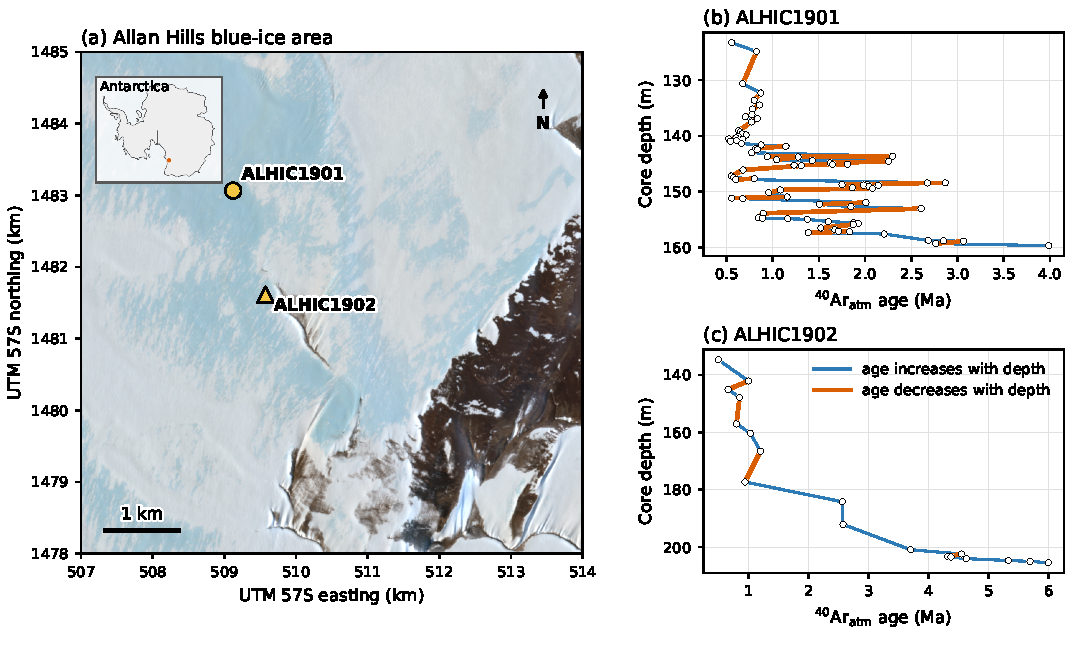
\includegraphics[width=\textwidth]{../figures/allan_hills_context.pdf}
\caption{\DIFaddFL{Allan Hills setting and published age--depth reversals. (a) Contrast-enhanced \(10~\mathrm{m}\) Copernicus Sentinel-2 L2A image acquired on 30 December 2025, with the locations of the two cores whose chronologies are plotted at right. The inset locates Allan Hills in Antarctica. (b) ALHIC1901 \(^{40}\mathrm{Ar}_{\mathrm{atm}}\) ages used in Figure~1b of \mbox{%DIFAUXCMD
\citet{MarksPeterson2026}}\hskip0pt%DIFAUXCMD
. (c) ALHIC1902 \(^{40}\mathrm{Ar}_{\mathrm{atm}}\) ages from \mbox{%DIFAUXCMD
\citet{Shackleton2025}}\hskip0pt%DIFAUXCMD
. Curves connect measurements in order of increasing depth; orange segments mark intervals where reported age decreases with depth. A decrease in age with depth establishes nonmonotonic core stratigraphy, but it implies an overturned continuous isochrone only if the samples belong to one continuous surface-deposited layer family. Core coordinates are from \mbox{%DIFAUXCMD
\citet{Shackleton2025}}\hskip0pt%DIFAUXCMD
.}}
\label{fig:allan-hills-context}
\end{figure}

\DIFaddend It remains unclear whether fixed topography in a steady glacier can generate a recumbent fold. Flow over topography produces layer draping or overriding \citep{Hindmarsh2006}, while rough-bed Stokes solutions can contain local extrusion (i.e., faster flow at depth) or, at greater slopes, separated circulation \citep{Gudmundsson1997linear,Gudmundsson1997nonlinear,Waddington2010}. Whether these motions reverse stratigraphic order is less clear.

Observed basal folds motivated a distinction between initiation and passive amplification. \citet{Hudleston1976} attributed Barnes Ice Cap folds to flow changes during minor advances or retreats, followed by bed-related shear. \citet{WhillansJohnsen1983} reproduced Byrd Station layer undulations using steady linear-viscous flow over basal variations, but did not obtain recumbent order reversal.

Airborne radar shows that order-reversing structures occur at ice-sheet scale. Dated horizons at Petermann Glacier contain overturned limbs and a sheath fold \citep{Bons2016}. Three-dimensional radar mapping in northeast Greenland resolved \(500\)--\(600~\mathrm{m}\) overturned anticline--syncline pairs associated with extinct ice streams \citep{Franke2022}. \citet{Franke2022} interpreted these structures as upright folds formed by earlier convergent flow and subsequently sheared into recumbent geometries after flow reorganization.

\citet{Waddington2001} examined whether local shear rotates a pre-existing wrinkle toward overturning or whether longitudinal extension flattens it, and argued that a transient process must first disturb steady stratigraphy. Finite-strain calculations later followed such inherited disturbances along trajectories and showed how divide migration can supply them \citep{JacobsonWaddington2004,JacobsonWaddington2005}. For continuously generated steady stratigraphy, \citet{ParreninHindmarshRemy2006} introduced logarithmic flux coordinates, and \citet{ParreninHindmarsh2007} generalized this construction to horizontally non-uniform velocity. Their \((\pi,\theta)\) coordinates (see Table~\ref{tab:notation} for notation)---the logarithms of total flux and normalized streamfunction---make steady particle trajectories parallel straight lines labelled by their surface origin \(\pi_0\). The associated path-sign parameter \(\alpha\) measures the change in separation between neighboring surface origins and shows that an isochrone passes through vertical when \(\alpha>1\). They proved that upward-increasing horizontal velocity precludes this state, but did not construct a glacier flow with \(\alpha>1\) or connect the criterion to full-Stokes mechanics. Their framework also supports vertical thinning functions and numerical age solvers \citep{Parrenin2013,HindmarshLeysingerVieliParrenin2009,ParreninChungMartin2025}.

Steady accumulation and near-surface flow can produce single-valued firn undulations \citep{NgKing2011,NgKing2013}, whereas traveling basal-traction anomalies produce overturned folds through an explicitly transient mechanism \citep{Wolovick2014,WolovickCreyts2016}. Full-Stokes models also amplify seeded or active structures through anisotropy, basal shear and bed relief \citep{Zhang2024}. Not every fold-like radar return traces a continuous surface-deposited isochrone. Steep specular limbs may be poorly imaged \citep{Holschuh2014}, and some northern Greenland structures contain debris-rich horizons with diffuse scattering \citep{Holschuh2026}. The unresolved step is whether a steady glacier velocity field can overturn the passive age field generated continuously at the surface. Table~\ref{tab:lineage} summarizes the relationship between these studies and the present analysis.

Here, we treat age as a passive, non-diffusive scalar introduced at surface deposition, and write the signed inverse vertical-thinning factor as the horizontal order of particles along an isochrone. Its cumulative budget separates surface-fast regular shear and extrusive reverse shear. We relate that budget to the full-Stokes stress balance, derive preservation regimes and obstacle bounds, and formulate \DIFdelbegin \DIFdel{a trajectory diagnostic. A gravity-driven full-Stokes example then overturns a surface-generated isochrone under a linear sliding law, without an inherited perturbation}\DIFdelend \DIFaddbegin \DIFadd{trajectory diagnostics. We then apply the direct tangent diagnostic to an incoming material line in a finite point-margin flow and to surface-deposited layers over periodic sinusoidal beds}\DIFaddend .

\section{Steady age transport and the order Jacobian}

\subsection{Kinematic coordinates and material origin}

Let \(u(x,z)\) and \(w(x,z)\) be the horizontal and vertical components of a continuously differentiable, steady two-dimensional velocity field in a domain bounded above by \(z=s(x)\). The flow is incompressible,
\begin{equation}
u_x+w_z=0.
\label{eq:incompressibility}
\end{equation}
After orienting \(x\) downstream, horizontal velocity remains positive along every trajectory considered:
\begin{equation}
u(x,z)>0.
\label{eq:forwardflow}
\end{equation}
Each trajectory intersects one upstream accumulation surface exactly once, at
\begin{equation}
x=x_0,
\qquad z=s(x_0),
\qquad \dot a(x_0)>0,
\label{eq:surfaceorigin}
\end{equation}
where \(\dot a\) is the ice-equivalent accumulation rate. Stratigraphic age is a passive, non-diffusive scalar that is zero at deposition and satisfies
\begin{equation}
\frac{\mathrm{D}\tau}{\mathrm{D}t}
=\underbrace{\tau_t}_{=0}+u\tau_x+w\tau_z
=u\tau_x+w\tau_z
=1,
\qquad \tau=0\quad\text{at deposition}.
\label{eq:age}
\end{equation}
The Eulerian age field is steady, so \(\tau_t=0\), although the age of a moving particle increases at one unit of time per unit time.

\DIFaddbegin \DIFadd{Equation~\ref{eq:age} is a first-order transport equation whose characteristics are particle trajectories. Along each characteristic, \(\mathop{}\!\mathrm{d}x/\mathop{}\!\mathrm{d}t=u\), \(\mathop{}\!\mathrm{d}z/\mathop{}\!\mathrm{d}t=w\) and \(\mathop{}\!\mathrm{d}\tau/\mathop{}\!\mathrm{d}t=1\), so age is the elapsed travel time from the deposition boundary. The surface coordinate \(x_0\) labels these characteristics, and the order Jacobian measures the sensitivity of their equal-age horizontal position to that initial label. The Jacobian analysis below is therefore the characteristic sensitivity of the steady age solution.
}

\DIFaddend Equations~\ref{eq:incompressibility} and \ref{eq:age} give the age--streamfunction Jacobian identity below. Equation~\ref{eq:forwardflow} permits integration in the downstream coordinate and excludes recirculation. Equation~\ref{eq:surfaceorigin} assigns every trajectory a unique deposition coordinate \(x_0\). Together they define a unique map from surface deposition to position on an isochrone and make the horizontal order Jacobian \(\left.\partial x/\partial x_0\right|_\tau\) well-defined. The discussion of steady overturning and limitations considers surface and basal sources, stagnation and other cases in which these conditions are not satisfied.

Equation~\ref{eq:incompressibility} permits the velocity to be represented by a scalar streamfunction \(\psi\). Curves of constant \(\psi\) are streamlines because \(\bm{u}\cdot\nabla\psi=0\), and the difference in \(\psi\) between two streamlines is their volume flux per unit width. The streamfunction is defined up to an arbitrary additive constant and requires no rheological assumption. We choose the orientation
\begin{equation}
 u=\psi_z,
 \qquad
 w=-\psi_x.
 \label{eq:streamfunction}
\end{equation}
Combining Equations~\ref{eq:age} and \ref{eq:streamfunction} gives the exact Jacobian identity
\begin{equation}
\begin{vmatrix}
\displaystyle\frac{\partial\tau}{\partial x} & \displaystyle\frac{\partial\tau}{\partial z} \\[1.2ex]
\displaystyle\frac{\partial\psi}{\partial x} & \displaystyle\frac{\partial\psi}{\partial z}
\end{vmatrix}
=\tau_x\psi_z-\tau_z\psi_x
=u\tau_x+w\tau_z
=1.
\label{eq:agepsiJacobian}
\end{equation}
Thus age and streamfunction form local area-preserving coordinates. Isochrones and streamlines intersect transversely wherever the assumptions hold. Equivalently, \((\tau,\psi)\) are local canonical coordinates in the sense of Hamiltonian mechanics: \(\psi\) is the Hamiltonian for particle trajectories and \(\{\tau,\psi\}=1\). The inverse transformation directly measures stratigraphic order. The appendix on inverse-coordinate identities gives the relations used below. Figure~\ref{fig:geometry} shows the deposition coordinate, two neighboring trajectories and their positions on an equal-age surface.

\begin{figure}[t]
\centering
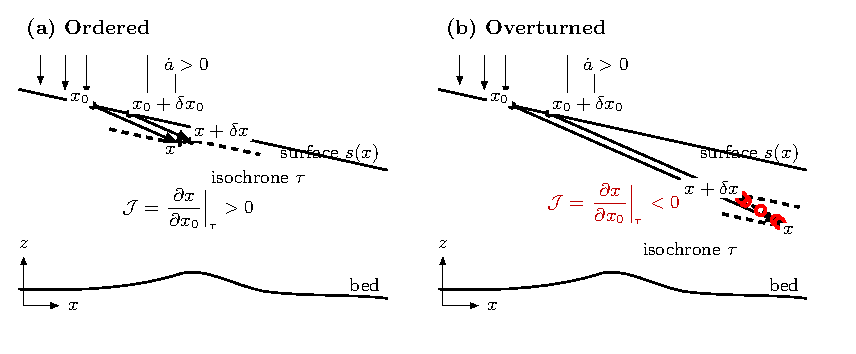
\includegraphics[width=\textwidth]{../figures/Figure1.pdf}
\caption{Material map for steady plane flow. Neighboring particles enter through the surface accumulation zone at \(x_0\) and \(x_0+\delta x_0\), follow distinct streamlines and reach positions separated by \(\delta x\) at the same age \(\tau\). The order Jacobian is the limit of \(\delta x/\delta x_0\). The curves enforce the kinematic requirements used in the derivation---surface origin, non-intersecting streamlines and transverse intersections with the isochrone---but are not a calculated Stokes solution.}
\label{fig:geometry}
\end{figure}

The streamfunction restricted to the surface is
\begin{equation}
\Psi(x)=\psi\bigl[x,s(x)\bigr].
\end{equation}
The steady surface kinematic condition is
\begin{equation}
 u_s s_x-\left.w\right|_{z=s(x)}=\dot a,
\label{eq:surfacekinematic}
\end{equation}
where \(u_s=u\bigl[x,s(x)\bigr]\). Differentiating \(\Psi\) with the chain rule, substituting Equation~\ref{eq:streamfunction}, and then applying Equation~\ref{eq:surfacekinematic} gives
\begin{equation}
\Psi'(x)
=\left.\psi_x\right|_{z=s(x)}+\left.\psi_z\right|_{z=s(x)}s_x
=-\left.w\right|_{z=s(x)}+u_ss_x
=\dot a(x)>0.
\label{eq:PsiPrime}
\end{equation}
The notation separates Eulerian position from material origin. The coordinate \(x\) is Eulerian: it identifies a fixed horizontal position in the steady velocity and age fields. The deposition coordinate \(x_0\) is a material-origin label that remains associated with a particle as it moves, although \(x_0\) alone labels a trajectory rather than a unique particle. At a specified age \(\tau\), \(x_0\) parameterizes the particles on an isochrone and therefore serves as the Lagrangian coordinate used below.

The label \(x_0\) is the physical-coordinate counterpart of the Parrenin--Hindmarsh coordinate \(\pi_0\): both identify a particle by its surface origin. Retaining \(x_0\) rather than transforming to logarithmic flux makes the present-day separation of neighboring origins directly measurable as a horizontal distance.

The streamfunction connects these descriptions. The increment \(\mathop{}\!\mathrm{d}\psi\) is the ice flux per unit width between neighboring streamlines. At the surface, this flux is \(\dot a_0\mathop{}\!\mathrm{d} x_0\), so larger accumulation places the same flux interval within a smaller deposition interval. Because \(\Psi'(x)>0\), every streamline label \(\psi\) has a unique deposition position \(x_0(\psi)\) satisfying
\begin{equation}
\Psi(x_0)=\psi,
\qquad
\frac{\mathop{}\!\mathrm{d} x_0}{\mathop{}\!\mathrm{d}\psi}=\frac{1}{\dot a_0},
\label{eq:x0psi}
\end{equation}
where \(\dot a_0\equiv\left.\dot a(x)\right|_{x=x_0}=\dot a(x_0)\) is the accumulation rate at deposition.

At fixed \(\psi\), Equation~\ref{eq:age} gives
\begin{equation}
\left.\frac{\partial\tau}{\partial x}\right|_{\psi}=\frac{1}{u}.
\end{equation}
Consequently the age at \((x,\psi)\) is the travel time from deposition. Here, \(\xi\) is the horizontal coordinate of integration and \(z(\xi,\psi)\) is the elevation of the streamline labelled by \(\psi\):
\begin{equation}
\tau(x,\psi)=\int_{x_0(\psi)}^{x}
\frac{\mathop{}\!\mathrm{d}\xi}{u\left[\xi,z(\xi,\psi)\right]}.
\label{eq:traveltime}
\end{equation}
At fixed \(x\), Equation~\ref{eq:streamfunction} implies
\begin{equation}
 z_{\psi}=\frac{1}{u}.
\label{eq:zpsi}
\end{equation}
Stratigraphic order compares travel times on neighboring streamlines, which are neighboring values of \(\psi\). We therefore differentiate Equation~\ref{eq:traveltime} with respect to \(\psi\) at fixed downstream position. Using Equations~\ref{eq:x0psi} and \ref{eq:zpsi} gives
\begin{equation}
\tau_{\psi}
=-\frac{1}{\dot a_0u_{s0}}
-\int_{x_0}^{x}\frac{u_z}{u^3}\,\mathop{}\!\mathrm{d}\xi,
\label{eq:taupsi}
\end{equation}
where \(u_{s0}=u\left[x_0,s(x_0)\right]\) is the horizontal speed at deposition. The first term records the separation imposed at deposition; the integral records the subsequent differential travel time between neighboring streamlines.

\subsection{Exact order theorem}

The material-origin coordinate records whether an isochrone retains its depositional ordering. Curvature alone is insufficient because a strongly curved isochrone can remain a single-valued depth surface and preserve the sequence of particles established at deposition. At fixed age, increasing \(x_0\) selects particles deposited successively farther downstream. Their order is preserved while their present horizontal position \(x\) also increases with \(x_0\); a vertical tangent occurs when this horizontal separation vanishes, and overturning begins when its sign reverses.

\medskip
\noindent\textbf{Definition 1 (Isochrone-order Jacobian).}
The isochrone-order Jacobian is
\begin{equation}
\mathcal{J}(x,x_0)
=\left.\frac{\partial x}{\partial x_0}\right|_{\tau}.
\label{eq:Jdefinition}
\end{equation}
It measures whether particles deposited in increasing order of \(x_0\) remain in increasing downstream order on an equal-age surface.

\medskip
\noindent\textbf{Theorem 1 (Cumulative order criterion).}
Under Equations~\ref{eq:incompressibility}--\ref{eq:age}, the isochrone-order Jacobian is
\begin{equation}
\boxed{
\mathcal{J}
=\frac{u(x,z)}{u_{s0}}
\left(
1+\dot a_0u_{s0}
\int_{x_0}^{x}\frac{u_z}{u^3}\,\mathop{}\!\mathrm{d}\xi
\right).
}
\label{eq:Jexact}
\end{equation}
It is also related exactly to the vertical age gradient by
\begin{equation}
\boxed{\mathcal{J}=-\dot a_0\tau_z.}
\label{eq:Jage}
\end{equation}
Hence \(\mathcal{J}>0\) denotes ordered stratigraphy, \(\mathcal{J}=0\) a vertical tangent, and \(\mathcal{J}<0\) an overturned limb.

\medskip
\noindent\textit{Proof.}
At fixed age, differentiation of \(\tau(x,\psi)\) gives
\begin{equation}
\left.\frac{\partial x}{\partial\psi}\right|_{\tau}
=-\frac{\tau_{\psi}}{\tau_x|_{\psi}}
=-u\tau_{\psi}.
\end{equation}
Multiplication by \(\mathop{}\!\mathrm{d}\psi/\mathop{}\!\mathrm{d} x_0=\dot a_0\) and substitution of Equation~\ref{eq:taupsi} gives Equation~\ref{eq:Jexact}. At fixed \(x\), \(\tau_z=\tau_{\psi}\psi_z=u\tau_{\psi}\), which gives Equation~\ref{eq:Jage}. \hfill\(\square\)

The correction of annual-layer thickness for cumulative ice deformation goes back at least to \citet{Nye1963} and \citet{DansgaardJohnsen1969}. In the present notation, the vertical thinning function \(\lambda_z\) is the current vertical thickness of an infinitesimal age layer divided by its ice-equivalent thickness at deposition. For an ordered layer, a positive age increment \(\mathop{}\!\mathrm{d}\tau\) corresponds to the present vertical thickness \(-\mathop{}\!\mathrm{d} z=-\mathop{}\!\mathrm{d}\tau/\tau_z\) and the initial thickness \(\dot a_0\mathop{}\!\mathrm{d}\tau\). Hence
\begin{equation}
\boxed{
\lambda_z
=-\frac{1}{\dot a_0\tau_z}
=\mathcal{J}^{-1},
\qquad \mathcal{J}>0.
}
\label{eq:thinningrelation}
\end{equation}
In ordered stratigraphy, \(\mathcal{J}\) is the inverse of the established vertical thinning function \citep{Parrenin2013,ParreninChungMartin2025}. Equation~\ref{eq:Jage} continues this measure with a sign through a vertical tangent. The positive thinning function diverges as \(\tau_z\rightarrow0\), whereas \(\mathcal{J}\) crosses zero regularly and records orientation reversal.

At deposition, \(x=x_0\), \(u=u_{s0}\), and \(\mathcal{J}=1\). At the first vertical tangent, \(\tau_z=0\), but the material curve remains regular. Inverting Equation~\ref{eq:agepsiJacobian} shows that
\begin{equation}
\left.\frac{\partial z}{\partial x_0}\right|_{\tau}
=\dot a_0\tau_x.
\end{equation}
When \(\mathcal{J}=0\), Equation~\ref{eq:age} gives \(\tau_x=1/u\), and therefore
\begin{equation}
\left.\frac{\partial z}{\partial x_0}\right|_{\tau,\mathcal{J}=0}
=\frac{\dot a_0}{u}>0.
\end{equation}
The divergence of the conventional slope \(m=\mathop{}\!\mathrm{d} z/\mathop{}\!\mathrm{d} x\) at overturning is therefore a coordinate singularity, not a singularity of the layer itself.

\subsection{Positive and reverse shear budgets}

Define
\begin{equation}
 u_z^+=\max(u_z,0),
 \qquad
 u_z^-=\max(-u_z,0),
\end{equation}
and the dimensionless cumulative contributions
\begin{align}
\mathcal{P}(x,x_0)
&=\dot a_0u_{s0}
\int_{x_0}^{x}\frac{u_z^+}{u^3}\,\mathop{}\!\mathrm{d}\xi,
\label{eq:Pdef}\\
\mathcal{R}(x,x_0)
&=\dot a_0u_{s0}
\int_{x_0}^{x}\frac{u_z^-}{u^3}\,\mathop{}\!\mathrm{d}\xi.
\label{eq:Rdef}
\end{align}
Equation~\ref{eq:Jexact} becomes
\begin{equation}
\boxed{
\mathcal{J}=\frac{u}{u_{s0}}\mathcal{B},
\qquad
\mathcal{B}\equiv1+\mathcal{P}-\mathcal{R}.
}
\label{eq:JPR}
\end{equation}
The dimensionless factor \(\mathcal{B}\) is an order budget: deposition contributes the initial value one, normal shear adds \(\mathcal{P}\), and reverse shear subtracts \(\mathcal{R}\). Because \(u/u_{s0}>0\), the necessary-and-sufficient condition for preservation of horizontal order is
\begin{equation}
\boxed{\mathcal{R}<1+\mathcal{P}.}
\label{eq:ordercondition}
\end{equation}
The first vertical tangent occurs at
\begin{equation}
\boxed{\mathcal{R}=1+\mathcal{P},}
\label{eq:verticalcondition}
\end{equation}
and overturning occurs when \(\mathcal{R}>1+\mathcal{P}\).

The unit term in Equations~\ref{eq:JPR}--\ref{eq:verticalcondition} represents the initial ordering imposed at deposition. Positive \(u_z\), the usual surface-fast glacier profile, adds to the budget. Reverse shear must remove both contributions. Thus a local region with \(u_z<0\) is not itself a fold criterion.

In travel-time coordinates, \(\mathop{}\!\mathrm{d} x=u\,\mathop{}\!\mathrm{d} t\), so
\begin{equation}
\mathcal{R}
=\dot a_0u_{s0}
\int_0^T\frac{u_z^-}{u^2}\,\mathop{}\!\mathrm{d} t.
\label{eq:Rtime}
\end{equation}
where \(T\) is the travel time from deposition to the point of interest. The contribution of reverse shear grows with residence time and as horizontal speed decreases. Local extrusion in fast throughflow may therefore leave stratigraphic order unchanged, while modest reverse shear near stagnation can dominate the order budget.

\medskip
\noindent\textbf{Corollary 1 (Monotonic-shear result).}
If \(u_z\geq0\) everywhere along a trajectory, then \(\mathcal{R}=0\), \(\mathcal{J}>0\), and the steady isochrone cannot overturn.

This corollary is the physical-coordinate statement of the no-overturning result in Appendix A of \citet{ParreninHindmarsh2007}. Finite intervals of reverse shear also preserve order when their cumulative weighted contribution remains below the budget in Equation~\ref{eq:ordercondition}. Figure~\ref{fig:budget} summarizes the three contributions and the point at which the budget reaches zero.

\begin{figure}[t]
\centering
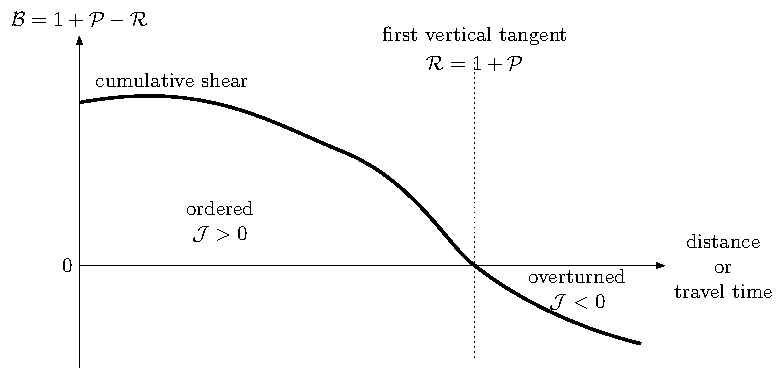
\includegraphics{../figures/Figure2.pdf}
\caption{Conceptual order budget. The sign of \(\mathcal{B}=1+\mathcal{P}-\mathcal{R}\) is the sign of the order Jacobian. Local reverse shear need not cause overturning; a vertical tangent appears only after cumulative reverse shear removes the initial depositional contribution and the accumulated normal-shear contribution.}
\label{fig:budget}
\end{figure}

\subsection{Relation to the Parrenin--Hindmarsh \((\pi,\theta)\) coordinates}

In the notation of \citet{ParreninHindmarsh2007}, \(Q(x)\) is total horizontal flux and \(\Omega\) is the streamfunction normalized by \(Q\). They defined
\begin{equation}
\pi=\ln\left[\frac{Q(x)}{Q^{\mathrm{ref}}}\right],
\qquad
\theta=\ln\Omega.
\end{equation}
Steady trajectories satisfy \(\mathop{}\!\mathrm{d}\theta/\mathop{}\!\mathrm{d}\pi=-1\), and hence \(\theta=\pi_0-\pi\). Curved trajectories in physical space therefore become parallel straight lines labelled by the deposition coordinate \(\pi_0\). For two neighboring particles, their Appendix A gives
\begin{equation}
\delta\pi=(1-\alpha)\,\delta\pi_0,
\end{equation}
where the path-sign parameter \(\alpha\) accumulates changes in the velocity profile along the trajectory. Thus \(1-\alpha\) is the signed deformation of neighboring surface origins in logarithmic flux coordinates, and an isochrone exceeds vertical when \(\alpha>1\). Their present and surface-origin coordinates are monotone functions of \(x\) and \(x_0\) wherever Equations~\ref{eq:forwardflow} and \ref{eq:surfaceorigin} hold. Consequently,
\begin{equation}
\operatorname{sgn}(1-\alpha)
=\operatorname{sgn}\!\left(
\left.\frac{\partial x}{\partial x_0}\right|_{\tau}
\right)
=\operatorname{sgn}(\mathcal{J})
=\operatorname{sgn}(-\tau_z).
\label{eq:PHsign}
\end{equation}
The order Jacobian carries the same sign information as \(1-\alpha\), and Equation~\ref{eq:thinningrelation} identifies it as the signed inverse vertical-thinning factor. In physical space, it separates the positive and negative parts of vertical shear, remains regular at the first vertical tangent and can be evaluated directly from a numerical velocity field.

\section{Full-Stokes constraints on isochrone order}

\subsection{Exact stress decomposition of vertical shear}

The order theorem applies to any velocity field satisfying the preceding kinematic equations. For steady, isothermal or thermomechanically prescribed, isotropic generalized-Newtonian Stokes flow, the momentum and constitutive equations constrain the vertical shear:
\begin{align}
\nabla\cdot\bm{u}&=0,
\label{eq:mass}\\
-\nabla p+\nabla\cdot\bm{\tau}+\rho\bm{g}&=\bm{0},
\label{eq:momentum}\\
\bm{\tau}&=2\eta\bm{D},
\qquad
\bm{D}=\tfrac12\left(\nabla\bm{u}+\nabla\bm{u}^{\mathsf T}\right),
\qquad \eta>0.
\label{eq:rheology}
\end{align}
Here, \(p\) is pressure, \(\rho\) is ice density, \(\bm{g}\) is gravitational acceleration, \(\bm{\tau}\) is deviatoric stress, \(\bm{D}\) is the strain-rate tensor and \(\eta>0\) is the scalar effective viscosity. The viscosity may depend on temperature and effective strain rate. Anisotropic rheology is discussed separately below.

With \(z\) vertical and gravity having no horizontal component, the horizontal momentum equation is
\begin{equation}
-p_x+\tau_{xx,x}+\tau_{xz,z}=0.
\label{eq:xmomentum}
\end{equation}
Write
\begin{equation}
p=p_{\mathrm{atm}}+\rho g(s-z)+p_{\mathrm{nh}},
\end{equation}
where \(g=|\bm{g}|\), \(p_{\mathrm{atm}}\) is atmospheric pressure and \(p_{\mathrm{nh}}\) contains all nonhydrostatic pressure, including the finite-slope surface correction. Integrating Equation~\ref{eq:xmomentum} downward from the free surface, with \(\zeta\) as the vertical coordinate of integration, gives
\begin{equation}
\tau_{xz}(x,z)
=\tau_{xz}^{s}
-\rho g s_x(s-z)
+\int_z^s\left(\tau_{xx,x}-p_{\mathrm{nh},x}\right)\,\mathop{}\!\mathrm{d}\zeta.
\label{eq:tauxzint}
\end{equation}
Because \(\tau_{xz}=\eta(u_z+w_x)\),
\begin{equation}
\boxed{
 u_z
 =\underbrace{\frac{\rho g(s-z)(-s_x)}{\eta}}_{G}
 +\underbrace{
 \left[
 -w_x+\frac{\tau_{xz}^{s}}{\eta}
 +\frac{1}{\eta}\int_z^s
 \left(\tau_{xx,x}-p_{\mathrm{nh},x}\right)\,\mathop{}\!\mathrm{d}\zeta
 \right]}_{R_{\mathrm{FS}}}.
}
\label{eq:uzdecomp}
\end{equation}
where the superscript \(s\) denotes surface stress. For a surface descending downstream, \(s_x\leq0\), the gravity-driven term \(G\) is nonnegative and favors order preservation. The residual \(R_{\mathrm{FS}}\) contains the full-Stokes effects omitted from the shallow-ice shear balance: gradients of vertical velocity, longitudinal stress, nonhydrostatic pressure and the Cartesian surface shear-stress component.

Substitution into Equation~\ref{eq:Jexact} gives
\begin{equation}
\mathcal{J}=\frac{u}{u_{s0}}
\left(1+\mathcal{G}+\mathcal{F}\right),
\label{eq:Jfullstokes}
\end{equation}
with
\begin{align}
\mathcal{G}&=\dot a_0u_{s0}
\int_{x_0}^{x}\frac{G}{u^3}\,\mathop{}\!\mathrm{d}\xi\geq0,
\label{eq:Ggrav}\\
\mathcal{F}&=\dot a_0u_{s0}
\int_{x_0}^{x}\frac{R_{\mathrm{FS}}}{u^3}\,\mathop{}\!\mathrm{d}\xi.
\label{eq:Gfs}
\end{align}
The exact full-Stokes condition for a vertical or overturned isochrone is
\begin{equation}
\boxed{
\mathcal{F}\leq-\left(1+\mathcal{G}\right).
}
\label{eq:FSfailure}
\end{equation}
A conservative sufficient condition for no overturning is
\begin{equation}
\boxed{
\dot a_0u_{s0}
\int_{x_0}^{x}
\frac{\left[R_{\mathrm{FS}}\right]_{-}}{u^3}\,\mathop{}\!\mathrm{d}\xi<1.
}
\label{eq:FSsufficient}
\end{equation}
This conservative bound is easy to test because it discards all positive contributions, including gravity-driven shear.

\subsection{Full-Stokes mechanics permits reverse shear}

Neither incompressibility nor the Stokes equations fixes the sign of \(u_z\). The constitutive relation constrains \(u_z+w_x\), while longitudinal stress and nonhydrostatic pressure can alter the Cartesian vertical gradient of horizontal speed. Analytical rough-bed solutions predict local velocity maxima and minima, and therefore regions with \(u_z<0\), even for gravity-driven linear viscous flow \citep{Gudmundsson1997linear}. The historical extrusion-flow literature likewise shows that surface-fast velocity profiles are not a pointwise theorem of full-Stokes mechanics \citep{Waddington2010}.

At stronger roughness, the one-way-flow assumption itself can fail. \citet{Gudmundsson1997nonlinear} found separated secondary circulation in troughs of sufficiently steep sinusoidal beds. \citet{Moffatt1964} considered the local similarity solution near a sharp corner. For two stationary rigid planes, the similarity exponent becomes complex when the included angle is less than approximately \(146^{\circ}\); the resulting oscillation with logarithmic radial distance gives a nested sequence of closed, counter-rotating streamlines. \citet{MeyerCreyts2017} extended this corner-flow mechanism to Glen-law ice in subglacial mountain valleys and showed that oblique flow can produce three-dimensional eddies.

Moffatt eddies require a recirculating corner-flow mode, whereas isochrone overturning \DIFdelbegin \DIFdel{under Equations~\ref{eq:incompressibility}--\ref{eq:age} requires the order budget along an open trajectory to reach zero. The circular-arc bed calculation in Figure~\ref{fig:positiveboundary} overturns with \(u>0\) along every plotted trajectory, so a Moffatt eddy is not necessary}\DIFdelend \DIFaddbegin \DIFadd{requires a signed material tangent to pass through vertical. The point-margin calculation below contains converging currents, but the plotted paths remain open and exit through the surface}\DIFaddend . A closed streamline is incompatible with the steady, surface-sourced age field: integrating Equation~\ref{eq:age} around an orbit of period \(T>0\) would give
\begin{equation*}
\tau(T)-\tau(0)
=
\int_0^T\frac{\mathrm{D}\tau}{\mathrm{D}t}\,\mathop{}\!\mathrm{d} t
=T,
\end{equation*}
although return to the same point requires \(\tau(T)=\tau(0)\). A Moffatt eddy may deform inherited layers or contain ice supplied by another boundary, but it cannot contain the steady surface-sourced age field considered here.

Published rough-bed solutions show that \(u_z\) can be negative. Order reversal further requires the integrated reverse-shear contribution \(\mathcal{R}\) to reach \(1+\mathcal{P}\).

\section{Regimes that preserve order}

\subsection{Shallow-ice flow}

Under the conventional shallow-ice approximation,
\begin{equation}
\tau_{xz}\simeq-\rho g(s-z)s_x.
\label{eq:SIAstress}
\end{equation}
For downstream flow with \(s_x<0\), \(\tau_{xz}>0\). An isotropic Glen-type rheology gives \(u_z\) with the same sign as \(\tau_{xz}\), while leading-order basal sliding contributes a depth-independent horizontal speed \citep{CuffeyPaterson2010}. Therefore
\begin{equation}
 u_z\geq0,
 \qquad \mathcal{R}=0,
 \qquad \mathcal{J}>0.
\label{eq:SIAorder}
\end{equation}
A fixed bed obstacle can produce arches, troughs and finite curvature in shallow-ice stratigraphy, but it cannot overturn a steady isochrone under these assumptions.

\subsection{Regular thin-film full-Stokes flow}

Let
\begin{equation}
\varepsilon=\frac{H}{L}\ll1
\end{equation}
be the aspect ratio of a smooth glacier. Higher-order glacier models reproduce the Stokes solution to second order in \(\varepsilon\) under their regular asymptotic assumptions, including a range of basal slip regimes \citep{Blatter1995,SchoofHindmarsh2010}. Suppose the non-shallow contribution scales as
\begin{equation}
R_{\mathrm{FS}}=O\left(\varepsilon^2\frac{U}{H}\right)
\label{eq:RFSscale}
\end{equation}
through a region of length \(L=H/\varepsilon\), and suppose \(u\) remains comparable to \(U\). Then
\begin{equation}
\mathcal{F}=O\left(\frac{\dot a}{U}\varepsilon\right).
\label{eq:GFSscale}
\end{equation}
Thus small regular full-Stokes corrections cannot erase the initial depositional contribution when
\begin{equation}
\frac{\dot a}{U}\varepsilon\ll1.
\label{eq:thinorder}
\end{equation}
This asymptotic regime excludes divides, abrupt sliding transitions, contact zones, steep obstacles, very slow flow and other regions where the thin-film expansion is singular or nonuniform.

\subsection{A sufficient bound for a localized obstacle}

The cumulative criterion bounds the effect of a localized obstacle without requiring pointwise monotonic shear.

\medskip
\noindent\textbf{Proposition 1 (Localized reverse-shear bound).}
Suppose reverse shear is confined to a trajectory segment of horizontal length \(\ell\). On that segment, assume
\begin{equation}
 u\geq U_{\min}>0,
 \qquad
 u_{s0}\leq U_{\mathrm{dep}},
 \qquad
 u_z^-\leq \dot\gamma_{\mathrm{rev}},
\label{eq:boundassumptions}
\end{equation}
where \(U_{\min}\) is the minimum horizontal speed on the segment, \(U_{\mathrm{dep}}\) bounds the horizontal speed at deposition, and \(\dot\gamma_{\mathrm{rev}}\) bounds the reverse vertical shear rate. Then
\begin{equation}
\boxed{
\mathcal{R}\leq
\frac{\dot a_0U_{\mathrm{dep}}\dot\gamma_{\mathrm{rev}}\ell}{U_{\min}^{3}}.
}
\label{eq:obstaclebound}
\end{equation}
A sufficient condition for no overturning is that the right-hand side be less than one.

\medskip
\noindent\textit{Proof.}
Substitute Equation~\ref{eq:boundassumptions} into Equation~\ref{eq:Rdef} and bound the integral by its maximum integrand multiplied by \(\ell\). \hfill\(\square\)

For an isolated obstacle whose horizontal and vertical influence scales are both \(O(H)\), with non-stagnant throughflow,
\begin{equation}
\mathcal{R}=O\left(\frac{\dot a}{U}\right).
\label{eq:isolatedscale}
\end{equation}
In a typical interior or flank setting where \(U\gg\dot a\), an isolated fixed bump can create local extrusion and visible draping while remaining far from the reverse-shear value required for a vertical tangent. More generally, setting the right-hand side of Equation~\ref{eq:obstaclebound} equal to one and solving for length gives
\begin{equation}
\ell
\gtrsim
\frac{U_{\min}^{3}}{\dot a_0U_{\mathrm{dep}}\dot\gamma_{\mathrm{rev}}}.
\label{eq:lengththreshold}
\end{equation}
Slow throughflow reduces this required length through the \(U_{\min}^{3}\) numerator. For scale, take \(\dot a_0=0.05~\mathrm{m\,yr^{-1}}\), \(U_{\mathrm{dep}}=10~\mathrm{m\,yr^{-1}}\), \(\dot\gamma_{\mathrm{rev}}=0.01~\mathrm{yr^{-1}}\) and \(\ell=1~\mathrm{km}\). Equation~\ref{eq:obstaclebound} gives \(\mathcal{R}\leq0.005\) when \(U_{\min}=10~\mathrm{m\,yr^{-1}}\), which rules out overturning under these assumed bounds. With \(U_{\min}=1~\mathrm{m\,yr^{-1}}\), the bound is \(\mathcal{R}\leq5\) and no longer rules it out.

For non-stagnant flow, localized deformation and a small accumulation-to-speed ratio, Equation~\ref{eq:obstaclebound} explains why flow over an isolated bump commonly preserves isochrone order.

\subsection{First-order cancellation over periodic roughness about plug flow}

Fixed periodic roughness can also have weak cumulative effect through cancellation about a plug-flow background. Let
\begin{equation}
 u(x,z;\epsilon_b)=U_b+\epsilon_b u_1(x,z)+O(\epsilon_b^2),
 \qquad U_b>0,
\label{eq:plugperturbation}
\end{equation}
where \(\epsilon_b\) is a small amplitude parameter, \(U_b>0\) is spatially uniform, \(u_1\) is periodic in \(x\), and \(k\) is its wavenumber. The perturbation has wavelength \(2\pi/k\) and zero horizontal mean at each elevation. Along the unperturbed trajectory \(z=z_0\),
\begin{equation}
\frac{u_z}{u^3}
=\epsilon_b\frac{u_{1,z}(x,z_0)}{U_b^3}+O(\epsilon_b^2).
\label{eq:periodicshear}
\end{equation}
Therefore, over one complete wavelength,
\begin{equation}
\int_{x}^{x+2\pi/k}\frac{u_z}{u^3}\,\mathop{}\!\mathrm{d}\xi=O(\epsilon_b^2).
\label{eq:periodiccancel}
\end{equation}
The appendix on first-order periodic cancellation gives the expansion leading to Equation~\ref{eq:periodiccancel}. The perturbative frictionless rough-bed solution of \citet{Gudmundsson1997linear} has this plug-flow structure: local extrusion occurs, but its first-order stoss- and lee-side contributions cancel over a complete symmetric wavelength.

The first-order cancellation in Equation~\ref{eq:periodiccancel} does not apply to a sheared background, a solitary asymmetric obstacle, a finite path ending mid-cycle, strongly nonlinear roughness or near-stagnant trajectories.

\section{Trajectory diagnostic for full-Stokes models}

The order criterion can be evaluated without explicitly solving the age equation or advecting a dense family of isochrones. Start trajectories in a surface accumulation zone and record \(x_0\), \(\dot a_0\) and \(u_{s0}\). With \(t\) denoting time since deposition, integrate along each trajectory
\begin{align}
\frac{\mathop{}\!\mathrm{d} x}{\mathop{}\!\mathrm{d} t}&=u,
&
\frac{\mathop{}\!\mathrm{d} z}{\mathop{}\!\mathrm{d} t}&=w,
\label{eq:trajectory}\\
\frac{\mathop{}\!\mathrm{d}\mathcal{P}}{\mathop{}\!\mathrm{d} t}
&=\dot a_0u_{s0}\frac{u_z^+}{u^2},
&
\frac{\mathop{}\!\mathrm{d}\mathcal{R}}{\mathop{}\!\mathrm{d} t}
&=\dot a_0u_{s0}\frac{u_z^-}{u^2},
\label{eq:PRode}
\end{align}
with \(\mathcal{P}(0)=\mathcal{R}(0)=0\). Then
\begin{equation}
\boxed{
\mathcal{J}(t)=\frac{u(t)}{u_{s0}}
\left[1+\mathcal{P}(t)-\mathcal{R}(t)\right].
}
\label{eq:Jdiagnostic}
\end{equation}
\DIFdelbegin \DIFdel{The }\DIFdelend \DIFaddbegin \DIFadd{Equations~\ref{eq:trajectory}--\ref{eq:Jdiagnostic} give a method-of-characteristics implementation of the age transport and its order sensitivity. Equation~\ref{eq:trajectory} traces a characteristic from the deposition boundary, Equation~\ref{eq:PRode} accumulates the signed shear history that controls separation from neighboring surface origins, and Equation~\ref{eq:Jdiagnostic} gives the resulting Jacobian without finite differencing neighboring trajectories.
}

\DIFadd{For prescribed material lines or geometries containing counterflow, we calculate signed local orientation directly from the deformation gradient. Let \(\bm{X}(t;\bm{X}_0)\) be the flow map and \(\bm{F}=\partial\bm{X}/\partial\bm{X}_0\). Along a steady characteristic,
}\begin{equation}
\DIFadd{\frac{\mathop{}\!\mathrm{d}\bm{X}}{\mathop{}\!\mathrm{d}t}=\bm{u}(\bm{X}),
\qquad
\frac{\mathop{}\!\mathrm{d}\bm{F}}{\mathop{}\!\mathrm{d}t}
=\nabla\bm{u}(\bm{X})\bm{F},
\qquad
\bm{F}(0)=\bm{I}.
\label{eq:deformationgradient}
}\end{equation}
\DIFadd{An initial material-line tangent \(\bm{T}_0=[1,m_0]^{\mathsf T}\) evolves as \(\bm{T}=\bm{F}\bm{T}_0\), so its signed horizontal-order metric is
}\begin{equation}
\DIFadd{\mathcal{J}_{\mathrm{T}}=T_x=F_{11}+m_0F_{12}.
\label{eq:tangentJ}
}\end{equation}
\DIFadd{For a surface-deposition characteristic, \(m_0=s_x(x_0)\) and Equation~\ref{eq:tangentJ} is the order Jacobian \(\mathcal{J}\). For a horizontal incoming material line, \(m_0=0\) and \(\mathcal{J}_{\mathrm{T}}=F_{11}\); this is a line-orientation metric rather than the surface-deposition Jacobian unless an upstream age boundary is supplied. The time-parameterized calculation contains no division by \(u\), remains regular when \(u=0\), and does not require a time-dependent layer simulation. Below, \(J\) denotes the applicable directly integrated metric in each numerical figure.
}

\DIFadd{For one-way, surface-sourced flow, the budget }\DIFaddend diagnostic is
\begin{equation}
\min_t\left[1+\mathcal{P}(t)-\mathcal{R}(t)\right]
\begin{cases}
>0, & \text{order preserved},\\
=0, & \text{first vertical tangent},\\
<0, & \text{overturned steady isochrone}.
\end{cases}
\label{eq:numericaltest}
\end{equation}

A robust implementation should include four checks. First, compare Equation~\ref{eq:Jdiagnostic} with \(-\dot a_0\tau_z\) from an independently solved steady age equation. Second, advect at least one pair of neighboring particles to verify the sign of \(\partial x/\partial x_0|_{\tau}\). Third, \DIFdelbegin \DIFdel{stop the downstream-coordinate integration when }\DIFdelend \DIFaddbegin \DIFadd{use Equation~\ref{eq:tangentJ} where }\DIFaddend \(u\) approaches zero \DIFaddbegin \DIFadd{or reverses, }\DIFaddend and diagnose recirculation with the full trajectory topology. Fourth, \DIFdelbegin \DIFdel{compute \(u_z\) using the finite-element gradient rather than differencing noisy interpolated velocities}\DIFdelend \DIFaddbegin \DIFadd{test the velocity-gradient calculation against interpolation, sampling and mesh resolution}\DIFaddend . Separate storage of \(\mathcal{P}\) and \(\mathcal{R}\) is preferable to integrating their difference because large compensating contributions can otherwise obscure numerical error.

For transient flow, Equation~\ref{eq:Jdiagnostic} is not valid because the steady travel-time representation fails. The \DIFdelbegin \DIFdel{corresponding calculation should integrate the deformation of the two-parameter deposition map through time . Nevertheless, the }\DIFdelend \DIFaddbegin \DIFadd{time-dependent analogue of Equation~\ref{eq:deformationgradient}, with \(\bm{u}=\bm{u}(\bm{X},t)\), remains valid, but the calculation must also retain deposition time in the two-parameter source map. The }\DIFaddend steady order budget remains useful as a baseline and as a diagnostic applied to quasi-steady snapshots.

\section{Full-Stokes numerical \DIFdelbegin \DIFdel{example}\DIFdelend \DIFaddbegin \DIFadd{experiments}\DIFaddend }

\DIFdelbegin \DIFdel{We construct an idealized steadyfull-Stokes flow that generates a recumbent fold from ordered surface deposition without an imposed internal disturbance. Gravity drives the flow, and the bed obeys a linear sliding law. The model is not a reconstruction of Allan Hills or another old-ice site.
}%DIFDELCMD <

%DIFDELCMD < %%%
\DIFdel{The two-dimensional domain has a flat }\DIFdelend \DIFaddbegin \DIFadd{Both experiments solve steady, incompressible, linear-viscous Stokes flow with \(\rho=917~\mathrm{kg\,m^{-3}}\), \(\eta=2.5\times10^8~\mathrm{Pa\,yr}\), a traction-free }\DIFaddend upper surface and \DIFdelbegin \DIFdel{a bed whose vertical cross section is a circular arc of radius \(250~\mathrm{m}\). Its maximum thickness is \(150~\mathrm{m}\), and it is truncated by vertical cuts where the ice has positive thickness. Ice is incompressible and linear viscous, with \(\eta=2.5\times10^8~\mathrm{Pa\,yr}\) and \(\rho=917~\mathrm{kg\,m^{-3}}\). Gravity acts at a mean surface slope of \(0.05~\mathrm{rad}\). We implemented the weak form in Firedrake version }\texttt{\DIFdel{0.13.0+11207.g7ed6ff028}}%DIFAUXCMD
\DIFdel{, generated curved unstructured meshes with Gmsh, imposed }\DIFdelend \DIFaddbegin \DIFadd{an impermeable bed obeying
}\begin{equation}
\DIFadd{u_t=C\tau_b,
\qquad
u_n=0,
\qquad
\tau_b=-\bm{t}\mathbin{\cdot}\bm{\sigma}\bm{n},
\label{eq:linearsliding}
}\end{equation}
\DIFadd{where \(C=10^{-5}~\mathrm{m\,yr^{-1}\,Pa^{-1}}\). We use Taylor--Hood elements, impose }\DIFaddend basal impermeability with symmetric Nitsche terms and \DIFdelbegin \DIFdel{solved the mixed system with the MUMPS direct solver. Velocity and pressure use Taylor--Hood elements, with quadratic velocityand linear pressure}\DIFdelend \DIFaddbegin \DIFadd{integrate the equivalent variational equation for \(\bm{F}\) or \(\bm{T}\) along characteristics of the computed velocity}\DIFaddend .

\DIFdelbegin \DIFdel{During model development, OpenAI }\texttt{\DIFdel{5.6-sol}} %DIFAUXCMD
\DIFdel{was used to search candidate boundary conditions, including bed geometry, for a clear example of steady overturning. The final geometry and boundary conditions were then evaluated using the governing equations, mechanical power balance, trajectory topology and mesh-refinement tests reported here.
}\DIFdelend \DIFaddbegin \subsection{\DIFadd{Finite convergent point-margin flow}}
\DIFaddend

\DIFdelbegin \DIFdel{The bed is impermeable and obeys the linear sliding law
}\begin{displaymath}
\DIFdel{u_t=C\tau_b,
\qquad
u_n=0,
\qquad
\tau_b=-\bm{t}\mathbin{\cdot}\bm{\sigma}\bm{n},
%DIFDELCMD < \label{eq:linearsliding}%%%
}\end{displaymath}%DIFAUXCMD
\DIFdel{where \(u_t\) }\DIFdelend \DIFaddbegin \DIFadd{The first experiment represents strong cross-sectional thickening and convergent flow near an exposed nunatak. It is a mechanism test rather than a reconstruction of Allan Hills. The domain is \(2~\mathrm{km}\) long, }\DIFaddend and \DIFdelbegin \DIFdel{\(u_n\) are the tangential and normal basal velocities, \(\bm{t}\) and \(\bm{n}\) are the bed tangent and outward normal, \(\bm{\sigma}\) is the full Cauchy stress, \(\tau_b\) is the resisting basal shear stress, and \(C=10^{-5}~\mathrm{m\,yr^{-1}\,Pa^{-1}}\) is the mobility. Because \(C>0\), Equation~\ref{eq:linearsliding} dissipates mechanical energy. The surface is traction free. Each lateral boundary has the hydrostatic traction \(-\rho g\cos\beta(-z)\bm{n}\), where \(\beta\) is the mean surface slope. The accumulation rate required to keep the surface fixed is diagnosed as \(\dot a=-\left.w\right|_{z=0}\), and particles are introduced only where \(\dot a>0\). }%DIFDELCMD <

%DIFDELCMD < %%%
\DIFdel{The numerical isochrones are generated from the deposition boundary. At age zero, a particle labelled by \(x_0\) is placed at \([x_0,0]^{\mathsf T}\). Integrating the steady velocity for a common age \(\tau\) gives the material curve \([x(x_0,\tau),z(x_0,\tau)]^{\mathsf T}\). No internal layer, wrinkle or fold is initialized. A negative value of \(\left.\partial x/\partial x_0\right|_\tau\) therefore measures order reversal generated between deposition and the plotted isochrone}\DIFdelend \DIFaddbegin \DIFadd{thickness increases smoothly from zero at the left point margin to \(360~\mathrm{m}\) at the right boundary. Surface slope changes from \(-0.035\) on the thin side to \(0.012\) on the thick side, producing rightward flow near the margin and leftward inflow from the thick side. Bed and surface meet at one point, so there is no left boundary facet or left flux. At the right boundary, \(u(z)\) is the linear-viscous SIA polynomial scaled to one percent of the reference SIA flux and \(w=0\). The surface remains traction free; its steady mass balance is therefore diagnosed from the computed normal velocity rather than prescribed}\DIFaddend .

\DIFdelbegin \DIFdel{For the representative calculation, the ice is \(70~\mathrm{m}\) thick at both lateral boundaries. The boundaries together remove \(4.3\times10^2~\mathrm{Pa\,m^2\,yr^{-1}}\) of mechanical power per unit width, whereas gravity supplies \(4.63\times10^6~\mathrm{Pa\,m^2\,yr^{-1}}\). The lateral tractions therefore do not drive the flow. The deposition map first reaches \(\mathcal{J}=-0.20\) at \(1.374~\mathrm{kyr}\) (Figure~\ref{fig:positiveboundary}a--b). At that age, all 47 surface origins spanning \(25.9~\mathrm{m}\) remain within the domain, and horizontal speed has remained above \(0.143~\mathrm{m\,yr^{-1}}\). The same threshold is reached with \(23\)--\(92~\mathrm{m}\) of ice at both boundaries }\DIFdelend \DIFaddbegin \DIFadd{Horizontal incoming lines overturn in this steady flow. The minimum sampled value is \(J=-0.1936\); restricting the inlet source height to \(\sigma_0\geq0.05\) still gives \(J=-0.0574\). The finite line shown in Figure~\ref{fig:nunatak-margin}e--f begins at \(\sigma_0=0.049\), first reaches \(J=0\) after \(130.2~\mathrm{kyr}\) and reaches \(J=-0.072\) after \(136.2~\mathrm{kyr}\). The point-margin value changes from \(-0.1946\) to \(-0.1934\) across the three meshes, and positive-thickness truncations converge toward the same result }\DIFaddend (Figure~\DIFdelbegin \DIFdel{\ref{fig:positiveboundary}c). }%DIFDELCMD <

%DIFDELCMD < %%%
\DIFdel{Horizontal speed remains positive along every plotted trajectory, so the streamlines are open and exclude a Moffatt eddy. Reverse shear rotates the surface-deposition map through vertical while the lateral ice thickness remains positive.
}%DIFDELCMD <

%DIFDELCMD < %%%
\DIFdel{For the \(70~\mathrm{m}\) boundary-thickness case, meshes with nominal spacings of \(15\), \(10\), \(7.5\) and \(5~\mathrm{m}\) give \(\mathcal{J}=-0.20061\), \(-0.20053\), \(-0.20040\) and \(-0.20037\), respectively, at the first resolved threshold. The overturned interval and its age are therefore insensitive to mesh refinement at the reported precision}\DIFdelend \DIFaddbegin \DIFadd{\ref{fig:nunatak-convergence}). A control imposing uniform surface ablation on the same geometry remains ordered, with \(J_{\min}=0.3075\); the reversal therefore depends on the surface-flux closure as well as geometry}\DIFaddend .

\begin{figure}[t]
\centering
\DIFdelbeginFL %DIFDELCMD < 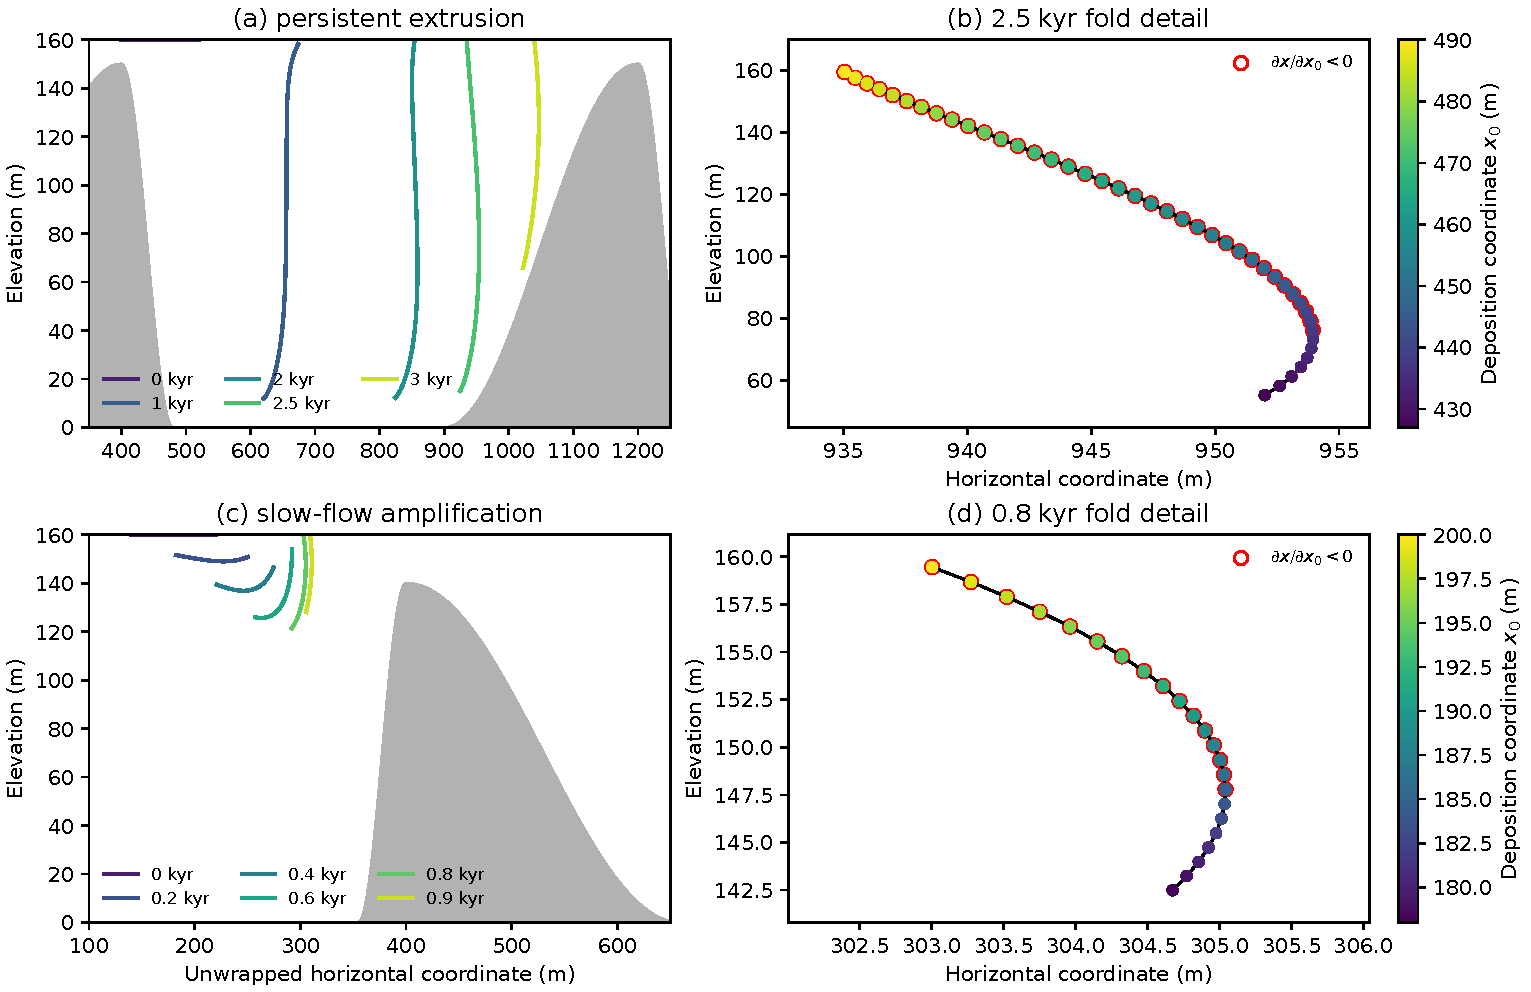
\includegraphics[width=\textwidth]{../figures/Figure3.pdf}
%DIFDELCMD < %%%
\DIFdelendFL \DIFaddbeginFL 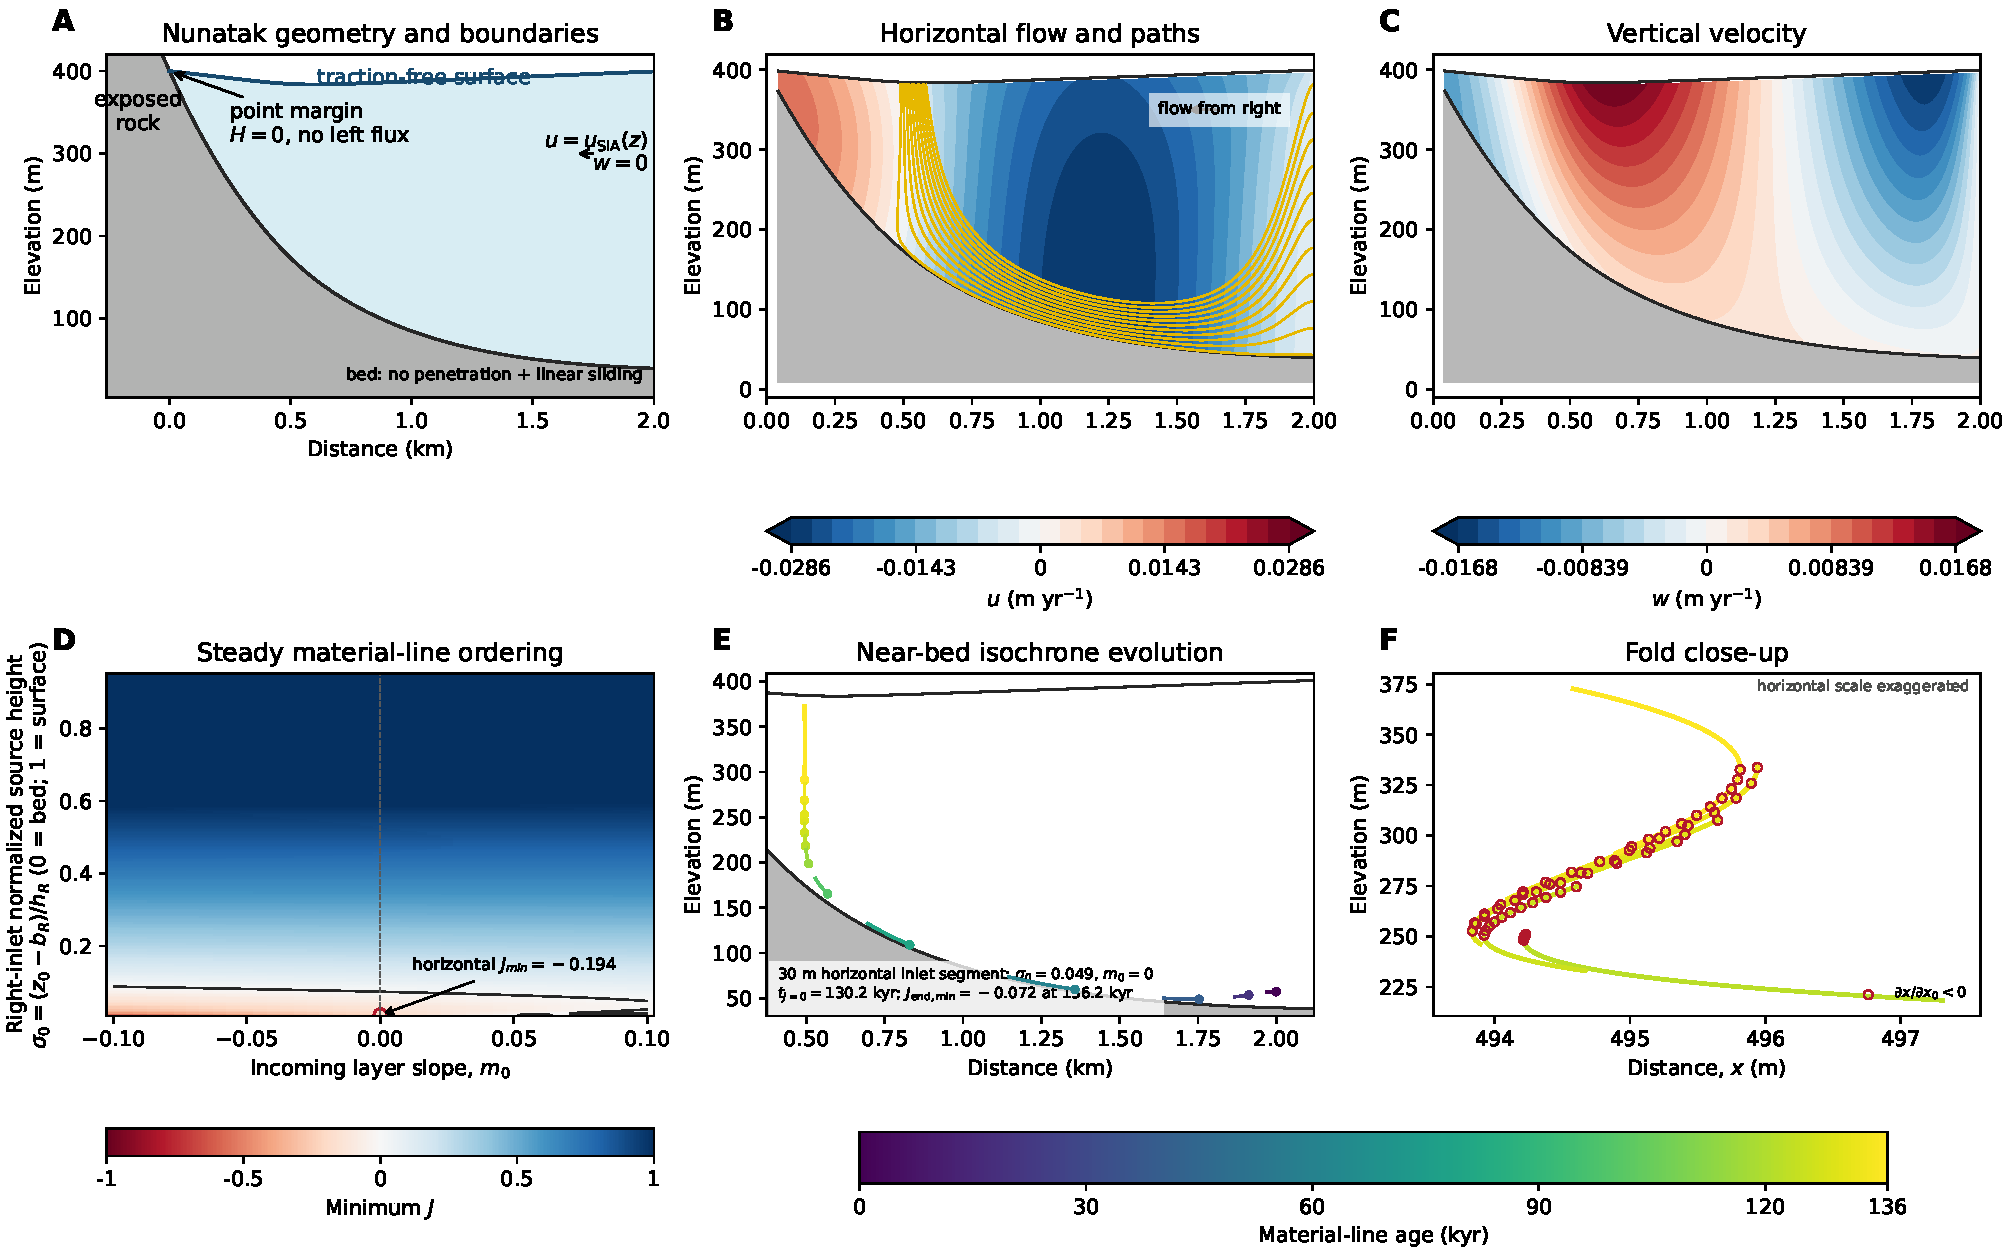
\includegraphics[width=\textwidth]{../figures/allan_hills_nunatak_margin.pdf}
\DIFaddendFL \caption{\DIFdelbeginFL \DIFdelFL{Gravity-driven order }\DIFdelendFL \DIFaddbeginFL \DIFaddFL{Steady }\DIFaddendFL reversal \DIFdelbeginFL \DIFdelFL{with positive thickness at both lateral boundaries}\DIFdelendFL \DIFaddbeginFL \DIFaddFL{of an incoming material line in a finite convergent point-margin flow}\DIFaddendFL . \DIFdelbeginFL \DIFdelFL{The bed cross section is }\DIFdelendFL \DIFaddbeginFL \DIFaddFL{(}\DIFaddendFL a\DIFdelbeginFL \DIFdelFL{circular arc with \(150~\mathrm{m}\) maximum ice thickness, }\DIFdelendFL \DIFaddbeginFL \DIFaddFL{) Geometry }\DIFaddendFL and \DIFaddbeginFL \DIFaddFL{boundary conditions. The right boundary has }\DIFaddendFL the \DIFdelbeginFL \DIFdelFL{bed obeys a linear sliding law}\DIFdelendFL \DIFaddbeginFL \DIFaddFL{plotted linear-viscous SIA-shaped horizontal inflow and \(w=0\)}\DIFaddendFL ; \DIFdelbeginFL \DIFdelFL{hydrostatic traction is applied on }\DIFdelendFL \DIFaddbeginFL \DIFaddFL{bed and surface meet at }\DIFaddendFL the \DIFdelbeginFL \DIFdelFL{open lateral cuts}\DIFdelendFL \DIFaddbeginFL \DIFaddFL{left point margin}\DIFaddendFL . (\DIFdelbeginFL \DIFdelFL{a}\DIFdelendFL \DIFaddbeginFL \DIFaddFL{b--c}\DIFaddendFL ) \DIFdelbeginFL \DIFdelFL{Isochrone evolution at \(0\), \(0.30\), \(0.60\), \(0.90\), \(1.15\) }\DIFdelendFL \DIFaddbeginFL \DIFaddFL{Horizontal velocity with selected paths }\DIFaddendFL and \DIFdelbeginFL \DIFdelFL{\(1.374~\mathrm{kyr}\), for \(70~\mathrm{m}\) boundary thickness}\DIFdelendFL \DIFaddbeginFL \DIFaddFL{vertical velocity}\DIFaddendFL . \DIFdelbeginFL \DIFdelFL{Each curve consists }\DIFdelendFL \DIFaddbeginFL \DIFaddFL{(d) Minimum tangent-order metric \(J=T_x\) over right-inlet source height \(\sigma_0=(z_0-b_R)/h_R\) and incoming slope \(m_0\). (e) Evolution }\DIFaddendFL of \DIFdelbeginFL \DIFdelFL{the same surface-deposition origins evaluated at }\DIFdelendFL a \DIFaddbeginFL \DIFaddFL{\(30~\mathrm{m}\) horizontal material segment initialized with a }\DIFaddendFL common age \DIFdelbeginFL \DIFdelFL{. (b) Detail at }\DIFdelendFL \DIFaddbeginFL \DIFaddFL{near }\DIFaddendFL the \DIFdelbeginFL \DIFdelFL{final age, when the minimum order Jacobian is less than \(-0.20\). Color }\DIFdelendFL \DIFaddbeginFL \DIFaddFL{right inlet; color }\DIFaddendFL gives \DIFdelbeginFL \DIFdelFL{deposition coordinate \(x_0\), and open red circles mark \(\mathcal{J}<0\)}\DIFdelendFL \DIFaddbeginFL \DIFaddFL{elapsed time}\DIFaddendFL . (\DIFdelbeginFL \DIFdelFL{c}\DIFdelendFL \DIFaddbeginFL \DIFaddFL{f}\DIFaddendFL ) \DIFdelbeginFL \DIFdelFL{Age }\DIFdelendFL \DIFaddbeginFL \DIFaddFL{Fold close-up; colored symbols mark segments with \(J_{\mathrm{T}}<0\) }\DIFaddendFL at \DIFdelbeginFL \DIFdelFL{which the same threshold }\DIFdelendFL \DIFaddbeginFL \DIFaddFL{successive elapsed times. This imposed inlet stratigraphy }\DIFaddendFL is \DIFdelbeginFL \DIFdelFL{crossed as boundary thickness increases }\DIFdelendFL \DIFaddbeginFL \DIFaddFL{not generated }\DIFaddendFL from \DIFdelbeginFL \DIFdelFL{\(23\) to \(92~\mathrm{m}\). All }\DIFdelendFL \DIFaddbeginFL \DIFaddFL{surface }\DIFaddendFL deposition \DIFdelbeginFL \DIFdelFL{origins remain in }\DIFdelendFL \DIFaddbeginFL \DIFaddFL{within }\DIFaddendFL the \DIFaddbeginFL \DIFaddFL{model }\DIFaddendFL domain\DIFdelbeginFL \DIFdelFL{at }\DIFdelendFL \DIFaddbeginFL \DIFaddFL{. The fixed, traction-free geometry diagnoses }\DIFaddendFL the \DIFdelbeginFL \DIFdelFL{plotted threshold}\DIFdelendFL \DIFaddbeginFL \DIFaddFL{surface mass balance required for steady closure}\DIFaddendFL . \DIFaddbeginFL \DIFaddFL{This idealized two-dimensional boundary-value problem is not an Allan Hills reconstruction.}\DIFaddendFL }
\DIFdelbeginFL %DIFDELCMD < \label{fig:positiveboundary}
%DIFDELCMD < %%%
\DIFdelendFL \DIFaddbeginFL \label{fig:nunatak-margin}
\label{fig:positiveboundary}% diff-only alias for references in deleted text
\DIFaddendFL \end{figure}

\DIFdelbegin \DIFdel{The topographic relief is large and the rheology is linear viscous. This idealized calculation gives a gravity-driven flow with a linear sliding law and positive lateral thickness that overturns a surface-generated isochrone. Testing the mechanism at Allan Hills requires measured three-dimensional geometry, a basal traction model and source-to-core trajectories consistent with the observed }\DIFdelend \DIFaddbegin \subsection{\DIFadd{Periodic sinusoidal-bed control}}

\DIFadd{The second experiment tests whether order reversal is generic to smooth bed roughness. One periodic cell has a flat surface and bed \(b(x)=-H+A\cos(2\pi x/\lambda)\); lateral boundaries are exactly periodic. Gravity is inclined at \(0.05~\mathrm{rad}\), and the }\DIFaddend surface mass balance \DIFaddbegin \DIFadd{\(\dot a=-w\) is diagnosed. Characteristics start on every accumulating surface interval, with the central \(80\%\) of its positive flux retained. Their initial tangent is horizontal, so \(J=T_x\)}\DIFaddend .

\DIFaddbegin \DIFadd{The sweep spans five mean thicknesses \(H=50\)--\(320~\mathrm{m}\), \(A/H=0\)--0.85 and \(\lambda/H=1/12\)--12. All 750 resolved numerical cases and 80 analytical flat-bed limits preserve order. The smallest resolved value is \(J=0.6428\) at \(H=50~\mathrm{m}\), \(A/H=0.85\) and \(\lambda/H=3\); the raw minimum through surface exit is 0.4428. Another 210 short-wave cells fall below the numerical surface-signal threshold and remain unclassified. Distortion is strongest at intermediate wavelength and weakens toward the resolved short- and long-wave limits (Figure~\ref{fig:sinusoidal-control}). Thus finite-amplitude symmetric roughness can strongly compress a surface-deposition map without overturning it over the resolved parameter range.
}

\begin{figure}[t]
\centering
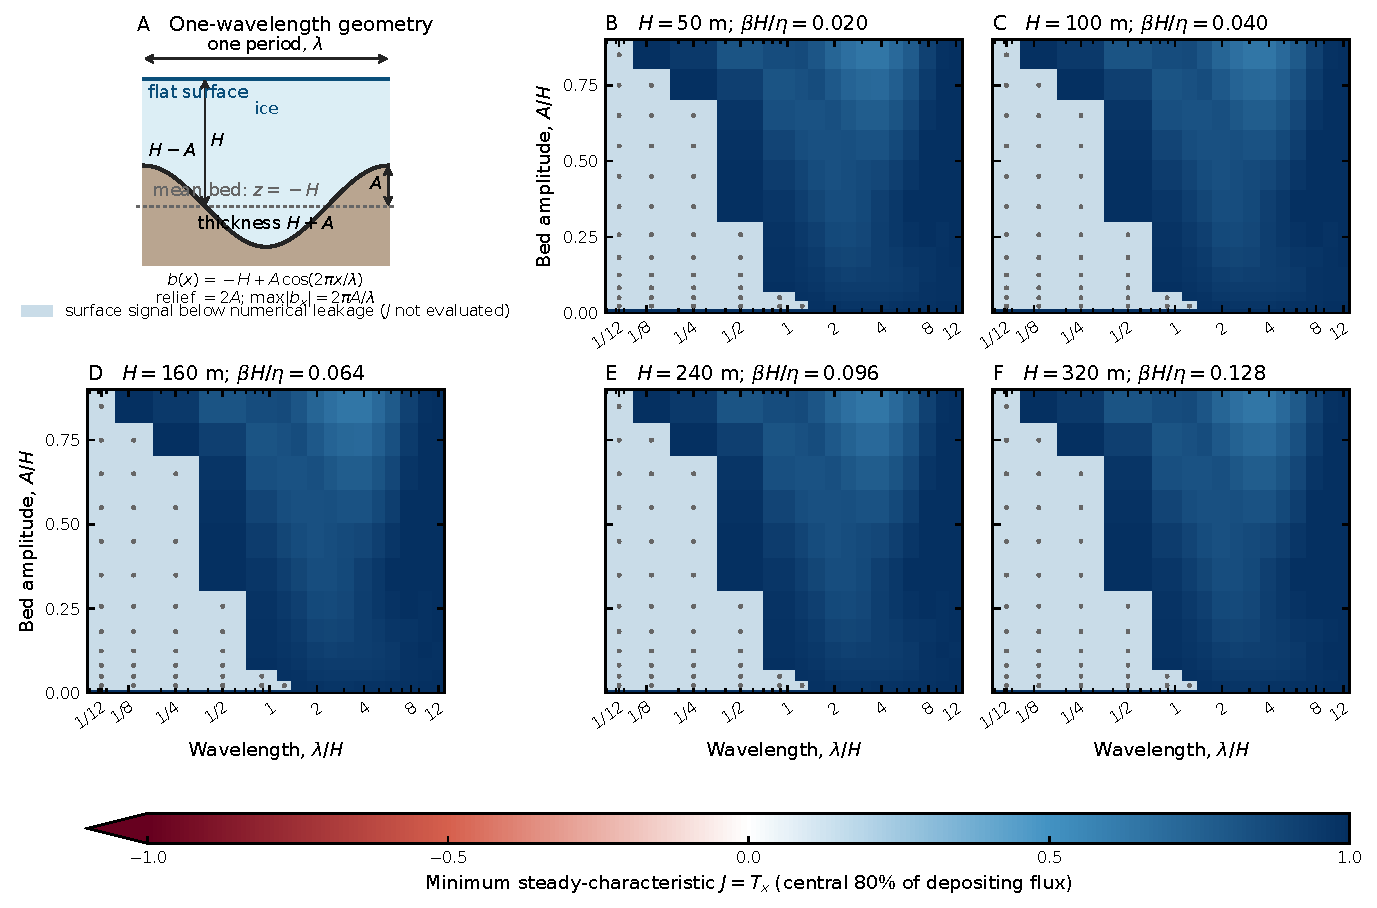
\includegraphics[width=\textwidth]{../figures/steady_characteristic_sinusoidal_parameter_map.pdf}
\caption{\DIFaddFL{Steady isochrone order over sinusoidal beds. (a) One periodic model cell with a flat surface and bed \(b(x)=-H+A\cos(2\pi x/\lambda)\). (b--f) Minimum order metric \(J=T_x\) for five mean thicknesses; \(\beta=C^{-1}\) and \(\beta H/\eta\) is the sliding-thickness ratio. Characteristics start on the physical surface wherever the diagnosed accumulation \(\dot a=-w\) is positive, retaining the central \(80\%\) of its flux. The primary diagnostic excludes only the upper \(5\%\) of local thickness beneath surface ablation. All 750 resolved numerical cells remain ordered, with \(J_{\min}=0.6428\); 80 flat-bed cells use the analytical limit \(J=1\). Dotted pale cells mark 210 cases whose surface signal is less than ten times the RMS basal normal leakage and are not evaluated. The dotted boundary marks numerical reach, not a physical transition.}}
\label{fig:sinusoidal-control}
\end{figure}

\DIFaddend \section{Discussion}

\subsection{Limits of the steady coordinate construction}

For flow satisfying Equations~\ref{eq:incompressibility}--\ref{eq:age}, cumulative reverse shear can overturn an isochrone when Equation~\ref{eq:verticalcondition} is met, without a change in boundary conditions. The extrusion-flow literature describes local reverse shear without evaluating this cumulative threshold. Variable density requires the mass-flux extension given in the appendix.

Stagnation and recirculation instead violate the coordinate construction. If \(u\) vanishes or reverses, downstream position no longer parameterizes a trajectory and the \(1/u\) and \(1/u^3\) integrals become singular. Time integration remains possible, but a closed streamline cannot have the unique surface origin assumed here. The Allan Hills model of \citet{Manos2026} approaches this limit: its near-stagnant basal flow remains nonzero, yet makes the order integral sensitive to small velocities.

Material sources also restrict the theorem. A trajectory may enter through accumulation and leave through surface ablation, but its deposition coordinate must be defined on the originating accumulation zone. Multiple surface sources or basal freeze-on require a more general label. Basal melting and ablation truncate layers, while freeze-on can add debris-bearing structures that are not surface-deposited isochrones \citep{LeysingerVieli2018,Holschuh2026}.

Changes in geometry or basal traction leave an inherited age field that differs from the steady age solution. Divide migration, traveling traction anomalies and former ice-stream configurations can therefore seed folds later amplified by shear \citep{JacobelBindschadler1993,JacobsonWaddington2005,Wolovick2014,WolovickCreyts2016,Franke2022,Jansen2024}. These mechanisms remain distinct from overturning generated continuously in a fixed velocity field.

Finally, Equation~\ref{eq:uzdecomp} assumes isotropic scalar viscosity and the order theorem is two-dimensional. Fabric and rheological heterogeneity can actively generate folds \citep{Alley1997,ThorsteinssonWaddington2002,Bons2016,Bons2025}, and convergent anisotropic flow occurs in both radar observations and models \citep{Ross2020,MartinGudmundssonPritchardGagliardini2009}. In three dimensions, the relevant quantity is the two-dimensional Jacobian mapping a surface deposition patch to an equal-age surface. The scalar \(\mathcal{J}\) applies only within a coherent flow tube with negligible cross-flow.

\subsection{Implications for old-ice sites}

Allan Hills approaches several limits of the two-dimensional calculation. Ice rises into an ablation zone above steep nunatak topography \citep{Spaulding2012,Kehrl2018,Stoll2026}. \citet{Manos2026} predict nearly stagnant basal ice upstream of the nunatak: the bottom \(20~\mathrm{m}\) averages \(0.4\)--\(0.5~\mathrm{mm\,yr^{-1}}\), with local speeds of order micrometres per year, compared with \(46\)--\(49~\mathrm{mm\,yr^{-1}}\) in the Cul-de-sac. Such small \(u\) makes the \(u^{-3}\) order integral numerically sensitive. The modeled flow is also three-dimensional, with bridging stresses represented in two dimensions by the \(-w_x\) term in Equation~\ref{eq:uzdecomp}. Finally, Cul-de-sac transport and geochemistry indicate a distinct accumulation environment.
\DIFdelbegin \DIFdel{A }\DIFdelend \DIFaddbegin

\DIFadd{The point-margin experiment represents the observed thick-ice-to-thin-ice convergence and shows that this boundary-value flow can reverse an imposed incoming material line. It neither tests the surface-deposition map nor predicts overturning at Allan Hills. A site calculation would require a }\DIFaddend three-dimensional, multi-source material map \DIFdelbegin \DIFdel{is therefore required there. }\DIFdelend \DIFaddbegin \DIFadd{built from measured geometry, basal traction and surface mass balance. Such a calculation would launch characteristics from each candidate accumulation source, follow them to the core or radar transect and evolve the two-dimensional Jacobian of the source patch. Equations~\ref{eq:deformationgradient}--\ref{eq:tangentJ} give the corresponding local calculation.
}\DIFaddend

Observations constrain but do not determine this history. The \(69^{\circ}\) mean dip in ALHIC2302 remains below vertical \citep{Kirkpatrick2025}, and centimetre-scale folds in ALHIC1901 need not explain core-scale reversals \citep{Stoll2026}. The ALHIC1901 age--depth inversion implies \(\mathcal{J}<0\) through Equation~\ref{eq:Jage} only if samples belong to one continuous surface-deposited layer family \citep{Shackleton2025}.

At Little Dome C, radar and flow modelling indicate strong basal thinning and possibly stagnant or disturbed ice \citep{Lilien2021,Chung2025BeyondEPICA}. Evaluating \(\mathcal{J}\) along trajectories would test whether steady flow preserves order above this basal unit.

The equations suggest four tests of an observed fold or age reversal.

\begin{enumerate}[leftmargin=*,label=(\arabic*)]
  \item \textbf{Steady geometry.} Evaluate \(\mathcal{P}\), \(\mathcal{R}\) and \(\mathcal{J}\) along source-to-core trajectories. A positive budget excludes steady overturning.
  \item \textbf{Flow topology and sources.} Test for stagnation, recirculation, freeze-on and multiple surface origins; these require the full material map.
  \item \textbf{Unsteady inheritance.} If steady flow preserves order, evaluate past changes in geometry, ablation and basal traction.
  \item \textbf{Active deformation.} If passive models underpredict folding, couple fabric and rheological heterogeneity to flow.
\end{enumerate}

In regular, shallow, non-stagnant flow, Equation~\ref{eq:obstaclebound} favors a time-dependent or rheological mechanism. \DIFdelbegin \DIFdel{More }\DIFdelend \DIFaddbegin \DIFadd{In more }\DIFaddend general full-Stokes flow\DIFdelbegin \DIFdel{can overturn steady isochrones if }\DIFdelend \DIFaddbegin \DIFadd{, the order criterion diagnoses overturning only if cumulative }\DIFaddend reverse shear crosses the \DIFdelbegin \DIFdel{order }\DIFdelend threshold.


\subsection{Novelty and relationship to established theory}

Studies of folding in rocks provide a useful comparison. Competence contrasts can drive active buckling, whereas passive layers record heterogeneous flow imposed by their surroundings; both processes can produce recumbent or sheath folds \citep{Bastida2014,SchmalholzMancktelow2016,NabaviFossen2021}. Recent fabric and field studies further show that similar sheath folds can reflect early active folding, later passive amplification, fold-axis rotation or a combination of these processes \citep{Fazio2024,AlsopCondon2025}. These studies generally describe the finite deformation of pre-existing layers. Here, \DIFdelbegin \DIFdel{isochrones are instead }\DIFdelend \DIFaddbegin \DIFadd{the analytical construction and sinusoidal control concern isochrones }\DIFaddend generated continuously at deposition, \DIFdelbegin \DIFdel{and we ask whether fixed steady flow can reverse that initially ordered map without an inherited disturbance or rheological contrast}\DIFdelend \DIFaddbegin \DIFadd{whereas the point-margin experiment tests the deformation of a prescribed incoming line}\DIFaddend .

The analysis builds most directly on the Parrenin--Hindmarsh \((\pi,\theta)\) coordinates, path-sign factor and monotonic-shear result \citep{ParreninHindmarshRemy2006,ParreninHindmarsh2007}. It also uses established material-line kinematics \citep{Waddington2001}, finite-strain amplification \citep{JacobsonWaddington2004}, vertical thinning \citep{Parrenin2013,ParreninChungMartin2025} and rough-bed extrusion \citep{Gudmundsson1997linear}. In physical space, the signed flux-coordinate mapping becomes a positive--negative \(u_z/u^3\) budget from which the full-Stokes residual threshold, localized-obstacle bound, periodic cancellation result and trajectory diagnostic follow.

\citet{ParreninHindmarshRemy2006} represented the horizontal velocity profile using a prescribed shape function of normalized depth, a separable approximation that enabled an analytical age solution. Their coordinate construction is more general than this profile. Here, the order theorem admits a general steady two-dimensional velocity field, and the full-Stokes momentum and constitutive equations determine the reverse shear that enters the order budget.

\DIFdelbegin \DIFdel{We are not aware of a previous full-Stokes calculation in which a time-independent glacier velocity }\DIFdelend \DIFaddbegin \DIFadd{The two numerical experiments test distinct source and boundary closures. The finite point-margin flow }\DIFaddend carries an ordered \DIFaddbegin \DIFadd{incoming line through \(J=0\), whereas the periodic sinusoidal beds preserve the }\DIFaddend surface-deposition map \DIFdelbegin \DIFdel{to \(\mathcal{J}<0\) without an internal wrinkle. In the present example, gravity drives the flow, a linear sliding law dissipates energy, lateral tractions are hydrostatic, and both lateral ice thickness and trajectory speed remain positive.
The circular-arc bed provides an idealized geometry for this mechanism.
}\DIFdelend \DIFaddbegin \DIFadd{throughout the resolved sweep. Their contrast bounds the scope of the mechanism but is not a controlled geometry-only comparison.
}\DIFaddend

Applying the diagnostic to reconstructed Allan Hills flow would distinguish a positive budget, which excludes steady overturning, from a trajectory crossing \(\mathcal{J}=0\). Layer attitudes, age reversals and fabric provide independent tests.

\subsection{Limitations}

The \DIFaddbegin \DIFadd{surface-deposition }\DIFaddend analysis assumes a smooth two-dimensional velocity, isotropic scalar viscosity and one surface origin per trajectory. The \DIFaddbegin \DIFadd{point-margin extension instead prescribes inlet stratigraphy and diagnoses a spatially varying surface mass balance; its line metric is not the surface-origin Jacobian. The }\DIFaddend obstacle bound requires externally supplied velocity and shear bounds, while periodic cancellation is only first order. The Jacobian \(\mathcal{J}\) diagnoses only a continuous material isochrone. Faults, unconformities, freeze-on, multiple sources and unresolved three-dimensional geometry can also produce apparent age reversals. Steep specular limbs or debris-rich diffuse reflectors add ambiguity in radar data \citep{Holschuh2014,Holschuh2026}.

\section{Conclusions}

The signed order Jacobian measures depositional order in a steady two-dimensional isochrone (Equation~\ref{eq:Jexact}). It is observable as \(-\dot a_0\tau_z\) (Equation~\ref{eq:Jage}) and, while positive, is the reciprocal of the established vertical thinning function (Equation~\ref{eq:thinningrelation}). The order budget separates the initial and normal-shear contributions from cumulative reverse shear; overturning begins when \(\mathcal{R}=1+\mathcal{P}\) (Equation~\ref{eq:verticalcondition}).

Full-Stokes mechanics permits reverse shear through longitudinal stress, nonhydrostatic pressure and horizontal gradients of vertical velocity (cf. Equation~\ref{eq:uzdecomp}). Shallow-ice flow preserves order (Equation~\ref{eq:SIAorder}), while localized obstacles and small-amplitude periodic roughness preserve it under the bounds in Equations~\ref{eq:obstaclebound} and \ref{eq:periodiccancel}. Stagnation and recirculation invalidate the one-way coordinate construction.

The \DIFdelbegin \DIFdel{numerical example generates a recumbent isochrone directly from ordered surface deposition }\DIFdelend \DIFaddbegin \DIFadd{finite point-margin experiment folds an ordered incoming material line }\DIFaddend (Figure~\DIFdelbegin \DIFdel{\ref{fig:positiveboundary}). Gravity drives the flow, the bed obeys a }\DIFdelend \DIFaddbegin \DIFadd{\ref{fig:nunatak-margin}), while the periodic sinusoidal-bed surface-deposition map remains ordered (Figure~\ref{fig:sinusoidal-control}). Both use the same }\DIFaddend linear sliding law, \DIFdelbegin \DIFdel{and both lateral ice thickness and horizontal velocity along the relevant trajectories remain positive. This steady full-Stokes flow crosses the order threshold under glaciological boundary conditions. }\DIFdelend \DIFaddbegin \DIFadd{but their source and boundary closures differ. Together they show that layer reversal is configuration dependent rather than a generic consequence of bed roughness.
}\DIFaddend

The order budget at old ice sites provides a common test of whether local flow preserves deposition order. Applying it requires reconstructed trajectories and, where cross-flow or multiple source regions are important, a three-dimensional material map. A fold complicates a climate archive, but it also preserves a mechanical record of the flow that brought ancient ice within reach.

\section*{Data availability statement}
No new observational data are presented. The \DIFaddbegin \DIFadd{published age--depth data in Figure~\ref{fig:allan-hills-context} are from the source data of \mbox{%DIFAUXCMD
\citet{Shackleton2025} }\hskip0pt%DIFAUXCMD
and \mbox{%DIFAUXCMD
\citet{MarksPeterson2026}}\hskip0pt%DIFAUXCMD
; the map uses Copernicus Sentinel-2 L2A imagery. The }\DIFaddend analytical results are fully specified by the equations in this manuscript. Executed notebooks \DIFaddbegin \DIFadd{and figure scripts }\DIFaddend contain the full-Stokes solves, trajectory calculations, numerical checks and figure generation and are available at \texttt{github.com/bradlipovsky/allan-hills-stratigraphy}.

\section*{Author contributions}
Bradley Paul Lipovsky developed the analysis and wrote the manuscript draft.

\section*{Competing interests}
None.

\section*{Acknowledgements}
The author received no funding from The Center for Old Ice Exploration (COLDEX), an NSF Science and Technology Center (NSF-2019719), for this work. The author nevertheless benefited from the Center's generous intellectual environment and is grateful for conversations with colleagues across its community.

OpenAI Codex using GPT-5 and \texttt{5.6-sol} (available at \texttt{openai.com/codex}) was used from 3 August to 1 September 2026 to assist with literature searches, drafting and revising manuscript text, LaTeX formatting, numerical-code development and the search for illustrative model geometries and boundary conditions. The author reviewed and revised all AI-assisted material, verified the cited sources, equations, code and numerical results, and takes full responsibility for the manuscript.

\bibliographystyle{igs}
\bibliography{references}

\appendix

\section{Notation}

\begingroup
\small
\begin{longtable}{@{}p{0.18\textwidth}p{0.59\textwidth}p{0.17\textwidth}@{}}
\caption{Notation. Units are given for \DIFdelbegin \DIFdel{the }\DIFdelend dimensional quantities used in the numerical \DIFdelbegin \DIFdel{example}\DIFdelend \DIFaddbegin \DIFadd{experiments}\DIFaddend ; all fluxes are ice-equivalent.}
\label{tab:notation}\\
\toprule
Symbol & Definition & Units \\
\midrule
\endfirsthead
\multicolumn{3}{@{}l}{\textit{Table~\ref{tab:notation} continued}}\\
\toprule
Symbol & Definition & Units \\
\midrule
\endhead
\bottomrule
\endfoot
\multicolumn{3}{@{}l}{\textit{Coordinates and kinematics}}\\
\(x,z\) & Horizontal and vertical Cartesian coordinates; \(x\) increases downstream. & \(\mathrm{m}\) \\
\(x_0\) & Horizontal coordinate of surface deposition; a material-origin label. & \(\mathrm{m}\) \\
\(\xi,\zeta\) & Horizontal and vertical coordinates of integration. & \(\mathrm{m}\) \\
\(z_0\) & Elevation of an unperturbed streamline in the periodic calculation. & \(\mathrm{m}\) \\
\(s(x)\) & Free-surface elevation. & \(\mathrm{m}\) \\
\(H,L,\ell\) & Ice thickness, horizontal forcing scale and length of a reverse-shear segment. & \(\mathrm{m}\) \\
\(t,\tau,T\) & Time since deposition, stratigraphic age and trajectory duration or orbit period. & \(\mathrm{yr}\) \\
\(\bm{u}=[u,w]^{\mathsf T}\) & Velocity vector and its horizontal and vertical components. & \(\mathrm{m\,yr^{-1}}\) \\
\DIFaddbegin \DIFadd{\(\bm{X},\bm{X}_0\) }& \DIFadd{Current and initial material positions in the flow map. }& \DIFadd{\(\mathrm{m}\) }\\
\DIFadd{\(\bm{F},\bm{T},m_0\) }& \DIFadd{Deformation gradient, material-line tangent and its initial slope. }& \DIFadd{\(1\) }\\
\DIFaddend \(u_s,u_{s0}\) & Horizontal surface speed and its value at deposition. & \(\mathrm{m\,yr^{-1}}\) \\
\(U,U_b\) & Characteristic horizontal speed and uniform background plug-flow speed. & \(\mathrm{m\,yr^{-1}}\) \\
\(U_{\min},U_{\mathrm{dep}}\) & Lower speed bound on a trajectory segment and upper bound on speed at deposition. & \(\mathrm{m\,yr^{-1}}\) \\
\(u_1\) & First-order horizontal-velocity perturbation. & \(\mathrm{m\,yr^{-1}}\) \\
\(\dot a,\dot a_0\) & Ice-equivalent surface accumulation rate and its value at \(x_0\). & \(\mathrm{m\,yr^{-1}}\) \\
\(\psi,\Psi\) & Streamfunction per unit width and its restriction to the surface, \(\Psi(x)=\psi[x,s(x)]\). & \(\mathrm{m^2\,yr^{-1}}\) \\
\(\delta x,\delta x_0\) & Horizontal separations at observation and deposition. & \(\mathrm{m}\) \\
\multicolumn{3}{@{}l}{\textit{Parrenin--Hindmarsh coordinates}}\\
\(Q,Q^{\mathrm{ref}}\) & Total horizontal flow-tube flux and its value at a reference position. & \(\mathrm{m^3\,yr^{-1}}\) \\
\(\Omega\) & Streamfunction normalized by total flux. & \(1\) \\
\(\pi,\theta\) & Logarithmic flux coordinates: \(\pi=\ln[Q(x)/Q^{\mathrm{ref}}]\) and \(\theta=\ln\Omega\). & \(1\) \\
\(\pi_0\) & Logarithmic flux coordinate of surface deposition. & \(1\) \\
\(\delta\pi,\delta\pi_0\) & Neighboring-particle separations in logarithmic flux at observation and deposition. & \(1\) \\
\(\alpha\) & Path-sign parameter defined by \(\delta\pi=(1-\alpha)\delta\pi_0\). & \(1\) \\
\multicolumn{3}{@{}l}{\textit{Stratigraphic order}}\\
\(\mathcal{J}\) & Isochrone-order Jacobian, \(\left.\partial x/\partial x_0\right|_\tau\). & \(1\) \\
\DIFaddbegin \DIFadd{\(\mathcal{J}_{\mathrm{T}}\) }& \DIFadd{Direct tangent-order metric, \(T_x=F_{11}+m_0F_{12}\). }& \DIFadd{\(1\) }\\
\DIFadd{\(\sigma_0\) }& \DIFadd{Normalized source height at the right inlet. }& \DIFadd{\(1\) }\\
\DIFaddend \(\lambda_z\) & Vertical thinning function for ordered stratigraphy. & \(1\) \\
\(u_z,u_z^+,u_z^-\) & Vertical shear and its positive and negative parts. & \(\mathrm{yr^{-1}}\) \\
\(\dot\gamma_{\mathrm{rev}}\) & Upper bound on reverse vertical shear. & \(\mathrm{yr^{-1}}\) \\
\(\mathcal{P},\mathcal{R}\) & Accumulated positive-shear and reverse-shear contributions. & \(1\) \\
\(\mathcal{B}\) & Order budget, \(1+\mathcal{P}-\mathcal{R}\). & \(1\) \\
\multicolumn{3}{@{}l}{\textit{Stress balance and asymptotic quantities}}\\
\(p,p_{\mathrm{atm}},p_{\mathrm{nh}}\) & Pressure, atmospheric pressure and nonhydrostatic pressure. & \(\mathrm{Pa}\) \\
\(\rho\) & Ice density. & \(\mathrm{kg\,m^{-3}}\) \\
\(\bm{g},g\) & Gravitational acceleration and its magnitude. & \(\mathrm{m\,s^{-2}}\) \\
\(\bm{\tau}\) & Deviatoric stress tensor; distinct from scalar age \(\tau\). & \(\mathrm{Pa}\) \\
\(\tau_{xx},\tau_{xz},\tau_{xz}^{s}\) & Longitudinal stress, shear stress and surface shear stress. & \(\mathrm{Pa}\) \\
\(\bm{D},\eta\) & Strain-rate tensor and scalar effective viscosity. & \(\mathrm{yr^{-1}},\ \mathrm{Pa\,yr}\) \\
\(G,R_{\mathrm{FS}}\) & Gravity-driven and residual full-Stokes contributions to \(u_z\). & \(\mathrm{yr^{-1}}\) \\
\(\mathcal{G},\mathcal{F}\) & Cumulative gravity-driven and residual full-Stokes order contributions. & \(1\) \\
\(\varepsilon\) & Glacier aspect ratio \(H/L\). & \(1\) \\
\(\epsilon_b,k\) & Roughness-amplitude parameter and horizontal wavenumber. & \(1,\ \mathrm{m^{-1}}\) \\
\DIFaddbegin \DIFadd{\(A,\lambda\) }& \DIFadd{Sinusoidal bed amplitude and wavelength. }& \DIFadd{\(\mathrm{m}\) }\\
\DIFaddend \multicolumn{3}{@{}l}{\textit{Numerical boundary condition}}\\
\(\bm{\sigma}\) & Full Cauchy stress tensor. & \(\mathrm{Pa}\) \\
\(\bm{t},\bm{n}\) & Unit tangent and outward unit normal on the bed. & \(1\) \\
\(u_t,u_n\) & Tangential and normal basal velocity components. & \(\mathrm{m\,yr^{-1}}\) \\
\(\tau_b,C\) & Resisting basal shear stress and linear-sliding mobility. & \(\mathrm{Pa},\ \mathrm{m\,yr^{-1}\,Pa^{-1}}\) \\
\DIFdelbegin \DIFdel{\(\beta\) }\DIFdelend \DIFaddbegin \DIFadd{\(\beta=C^{-1}\) }\DIFaddend & \DIFdelbegin \DIFdel{Mean surface slope used to orient gravity in the numerical example}\DIFdelend \DIFaddbegin \DIFadd{Linear basal-drag coefficient}\DIFaddend . & \DIFdelbegin \DIFdel{\(\mathrm{rad}\) }\DIFdelend \DIFaddbegin \DIFadd{\(\mathrm{Pa\,yr\,m^{-1}}\) }\DIFaddend \\
\multicolumn{3}{@{}l}{\textit{Operators and conventions}}\\
\((\,\cdot\,)_x,(\,\cdot\,)_z,(\,\cdot\,)_t\) & Partial derivatives with respect to \(x,z,t\); \(u_t\) instead denotes tangential velocity where explicitly stated. & --- \\
\(\mathrm{D}/\mathrm{D}t,\nabla\) & Material time derivative and spatial gradient. & --- \\
\((\,\cdot\,)^{\mathsf T},\{\,\cdot\,,\,\cdot\,\}\) & Transpose and Poisson bracket. & --- \\
\(\left.\partial(\,\cdot\,)/\partial x\right|_\psi\) & Partial derivative with the subscripted coordinate held fixed; analogous notation is used for other variables. & --- \\
\([f]_{-}\) & Negative-part magnitude, \(\max(-f,0)\). & units of \(f\) \\
\(\operatorname{sgn},\det,O(\,\cdot\,)\) & Sign, determinant and asymptotic-order notation. & --- \\
\end{longtable}
\endgroup

\section{Relationship to previous studies}

\begingroup
\scriptsize
\setlength{\aboverulesep}{0.2ex}
\setlength{\belowrulesep}{0.2ex}
\begin{longtable}{@{}p{0.20\textwidth}p{0.37\textwidth}p{0.37\textwidth}@{}}
\caption{Relationship between established folding analyses and the present formulation.}
\label{tab:lineage}\\
\toprule
Study & Primary question & Diagnostic and scope \\
\midrule
\endfirsthead
\multicolumn{3}{@{}l}{\textit{Table~\ref{tab:lineage} continued}}\\
\toprule
Study & Primary question & Diagnostic and scope \\
\midrule
\endhead
\bottomrule
\endfoot
\citet{Hudleston1976} & How did observed basal recumbent folds form? & A transient change in flow creates misalignment, followed by passive amplification over an irregular bed. \\
\midrule
\citet{WhillansJohnsen1983} & How do fixed basal variations distort radar layers? & Linear-viscous flow over relief with variable sliding and drag; calculated undulations match Byrd Station radar layers. \\
\midrule
\citet{Waddington2001} & Does a pre-existing local wrinkle flatten or rotate toward overturning? & Instantaneous tangent slope relative to a steady reference isochrone. \\
\midrule
\citet{JacobsonWaddington2004} & Does a finite-strain history overturn an injected disturbance? & Deformation gradient integrated along trajectories. \\
\midrule
\citet{ParreninHindmarshRemy2006,ParreninHindmarsh2007} & How does steady flow shape isochrones and preserve particle order? & Log total flux and log normalized streamfunction straighten trajectories; the path-sign factor maps deposition coordinate \(\pi_0\) to present coordinate \(\pi\). \\
\midrule
\citet{NgKing2011,NgKing2013} & Can steady spatial forcing generate folded firn geometry? & Accumulation and near-surface flow generate single-valued layer undulations, but not recumbent order reversal. \\
\midrule
\citet{Bons2016,Franke2022} & What do three-dimensional radar surveys show about large folds? & Dated horizons contain overturned and sheath folds that record convergence, basal shear and former flow configurations. \\
\midrule
\citet{Wolovick2014,WolovickCreyts2016} & Can changing basal traction generate observed overturning? & Traveling slippery or sticky patches produce thickness-scale overturned folds. \\
\midrule
\citet{Hindmarsh2006} & Do layers drape or override bed and basal-boundary perturbations? & Perturbation and full-mechanical models; wavelength controls architecture. \\
\midrule
\citet{Zhang2024} & How do anisotropy, convergent flow and bed relief amplify englacial folds? & Full-Stokes growth of active or bed-seeded structures, including recumbent basal folds. \\
\midrule
\citet{HindmarshLeysingerVieliParrenin2009,ParreninChungMartin2025} & How can age and thinning be computed accurately in steady flow tubes? & Eulerian and characteristic solvers for age, origin and vertical thinning. \\
\midrule
\citet{Gudmundsson1997linear} & Can rough-bed Stokes flow contain local extrusion? & Analytical velocity extrema and reverse vertical shear near sinusoidal relief. \\
\midrule
This study & Has cumulative reverse shear erased depositional ordering? & Signed inverse-thinning factor, positive--negative shear budget, full-Stokes threshold, obstacle bounds and trajectory diagnostic. \\
\end{longtable}
\endgroup

\section{Inverse-coordinate identities}

Equation~\ref{eq:agepsiJacobian} can be written
\begin{equation}
\begin{bmatrix}
\tau_x & \tau_z\\
\psi_x & \psi_z
\end{bmatrix}
\begin{bmatrix}
\mathop{}\!\mathrm{d} x\\
\mathop{}\!\mathrm{d} z
\end{bmatrix}
=
\begin{bmatrix}
\mathop{}\!\mathrm{d}\tau\\
\mathop{}\!\mathrm{d}\psi
\end{bmatrix},
\qquad
\det=1.
\end{equation}
The inverse transformation is
\begin{equation}
\begin{bmatrix}
\mathop{}\!\mathrm{d} x\\
\mathop{}\!\mathrm{d} z
\end{bmatrix}
=
\begin{bmatrix}
\psi_z & -\tau_z\\
-\psi_x & \tau_x
\end{bmatrix}
\begin{bmatrix}
\mathop{}\!\mathrm{d}\tau\\
\mathop{}\!\mathrm{d}\psi
\end{bmatrix}
=
\begin{bmatrix}
 u & -\tau_z\\
 w & \tau_x
\end{bmatrix}
\begin{bmatrix}
\mathop{}\!\mathrm{d}\tau\\
\mathop{}\!\mathrm{d}\psi
\end{bmatrix}.
\label{eq:inversemap}
\end{equation}
Therefore
\begin{equation}
 x_{\tau}|_{\psi}=u,
 \quad
 z_{\tau}|_{\psi}=w,
 \quad
 x_{\psi}|_{\tau}=-\tau_z,
 \quad
 z_{\psi}|_{\tau}=\tau_x.
\end{equation}
The first two identities state that advancing one unit in age at fixed streamline follows the velocity for one unit of time. The latter two specify the equal-age tangent. Multiplication by \(\mathop{}\!\mathrm{d}\psi/\mathop{}\!\mathrm{d} x_0=\dot a_0\) yields Equation~\ref{eq:Jage} and the corresponding vertical tangent component.

\section{Extension to steady variable-density flow}

Below the firn, glacier ice is commonly approximated as incompressible with nearly constant density \citep{lipovsky2022density}. The coordinate construction extends to a steady variable-density flow satisfying
\begin{equation}
\nabla\cdot(\rho\bm{u})=0.
\end{equation}
Define the mass-flux streamfunction by
\begin{equation}
\rho u=\psi_z,
\qquad
\rho w=-\psi_x.
\end{equation}
Then
\begin{equation}
\begin{vmatrix}
\tau_x & \tau_z \\
\psi_x & \psi_z
\end{vmatrix}
=\rho(u\tau_x+w\tau_z)=\rho.
\end{equation}
The mapping remains nonsingular for \(\rho>0\), and the same order interpretation follows after replacing volume flux by mass flux. The constant-density formula therefore extends to positive variable density, with density factors in the cumulative weights.

\section{First-order periodic cancellation about plug flow}

Let
\begin{equation}
 u(x,z;\epsilon_b)=U_b+\epsilon_b u_1(x,z)+O(\epsilon_b^2),
 \qquad U_b>0,
\end{equation}
where \(U_b\) is spatially uniform and \(u_1\) is periodic in \(x\) with wavelength \(2\pi/k\) and zero horizontal mean at each elevation. Then
\begin{equation}
 u_z=\epsilon_b u_{1,z}+O(\epsilon_b^2),
 \qquad
 u^{-3}=U_b^{-3}+O(\epsilon_b).
\end{equation}
Because the background integrand is identically zero, the \(O(\epsilon_b)\) displacement of the trajectory affects the integral only at \(O(\epsilon_b^2)\). Evaluating the first-order term along the unperturbed streamline \(z=z_0\) gives
\begin{equation}
\int_x^{x+2\pi/k}\frac{u_z}{u^3}\,\mathop{}\!\mathrm{d}\xi
=\frac{\epsilon_b}{U_b^3}
\int_x^{x+2\pi/k}u_{1,z}(\xi,z_0)\,\mathop{}\!\mathrm{d}\xi
+O(\epsilon_b^2)
=O(\epsilon_b^2),
\end{equation}
because differentiation with respect to \(z\) preserves the zero horizontal mean of \(u_1\), giving Equation~\ref{eq:periodiccancel}. For a vertically sheared background, trajectory displacement can act on the nonzero background integrand at first order, so the cancellation does not follow without additional assumptions.
\DIFaddbegin

\clearpage
\setcounter{figure}{0}
\renewcommand{\thefigure}{S\arabic{figure}}
\section{\DIFadd{Point-margin numerical convergence}}

\begin{figure}[h]
\centering
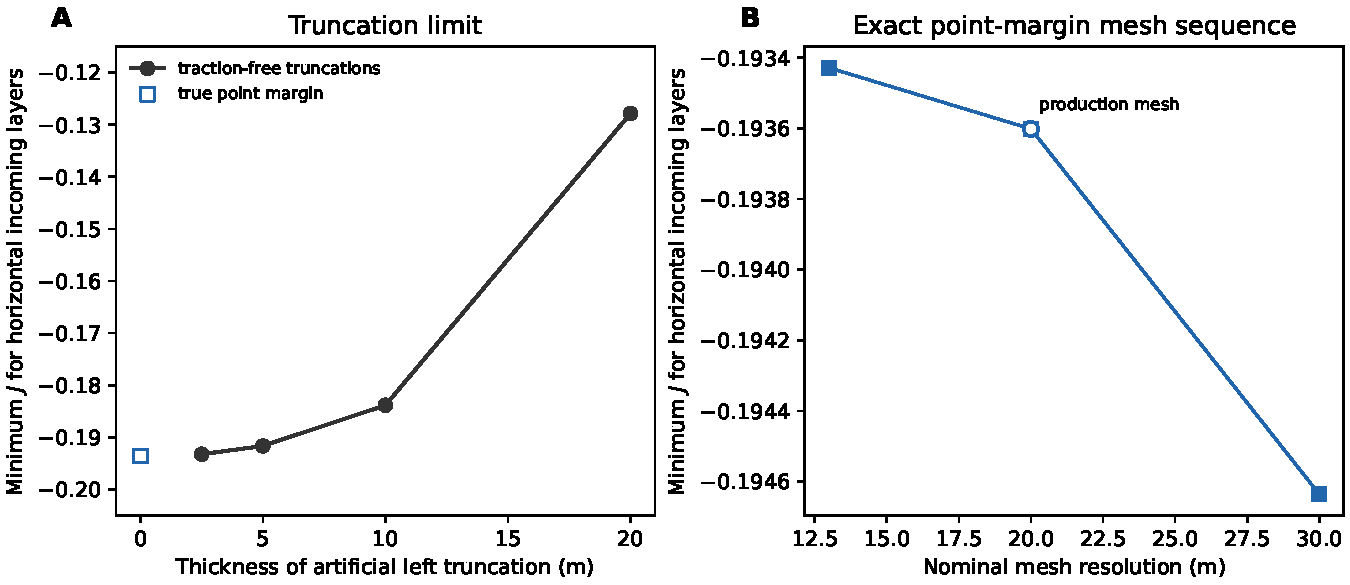
\includegraphics[width=0.92\textwidth]{../figures/allan_hills_nunatak_margin_convergence.pdf}
\caption{\DIFaddFL{Numerical checks for the finite convergent point-margin experiment. (a) Minimum \(J\) for horizontal incoming lines as an artificial traction-free left truncation decreases from \(20~\mathrm{m}\) thickness toward the true point margin. (b) Exact point-margin result across three nominal mesh resolutions; the open symbol marks the production mesh used in Figure~\ref{fig:nunatak-margin}. Every value remains negative.}}
\label{fig:nunatak-convergence}
\end{figure}
\DIFaddend

\end{document}
